\section{Tree\-Model Class Reference}
\label{classTreeModel}\index{TreeModel@{TreeModel}}
{\tt \#include $<$treemodel.h$>$}

Inheritance diagram for Tree\-Model:\begin{figure}[H]
\begin{center}
\leavevmode
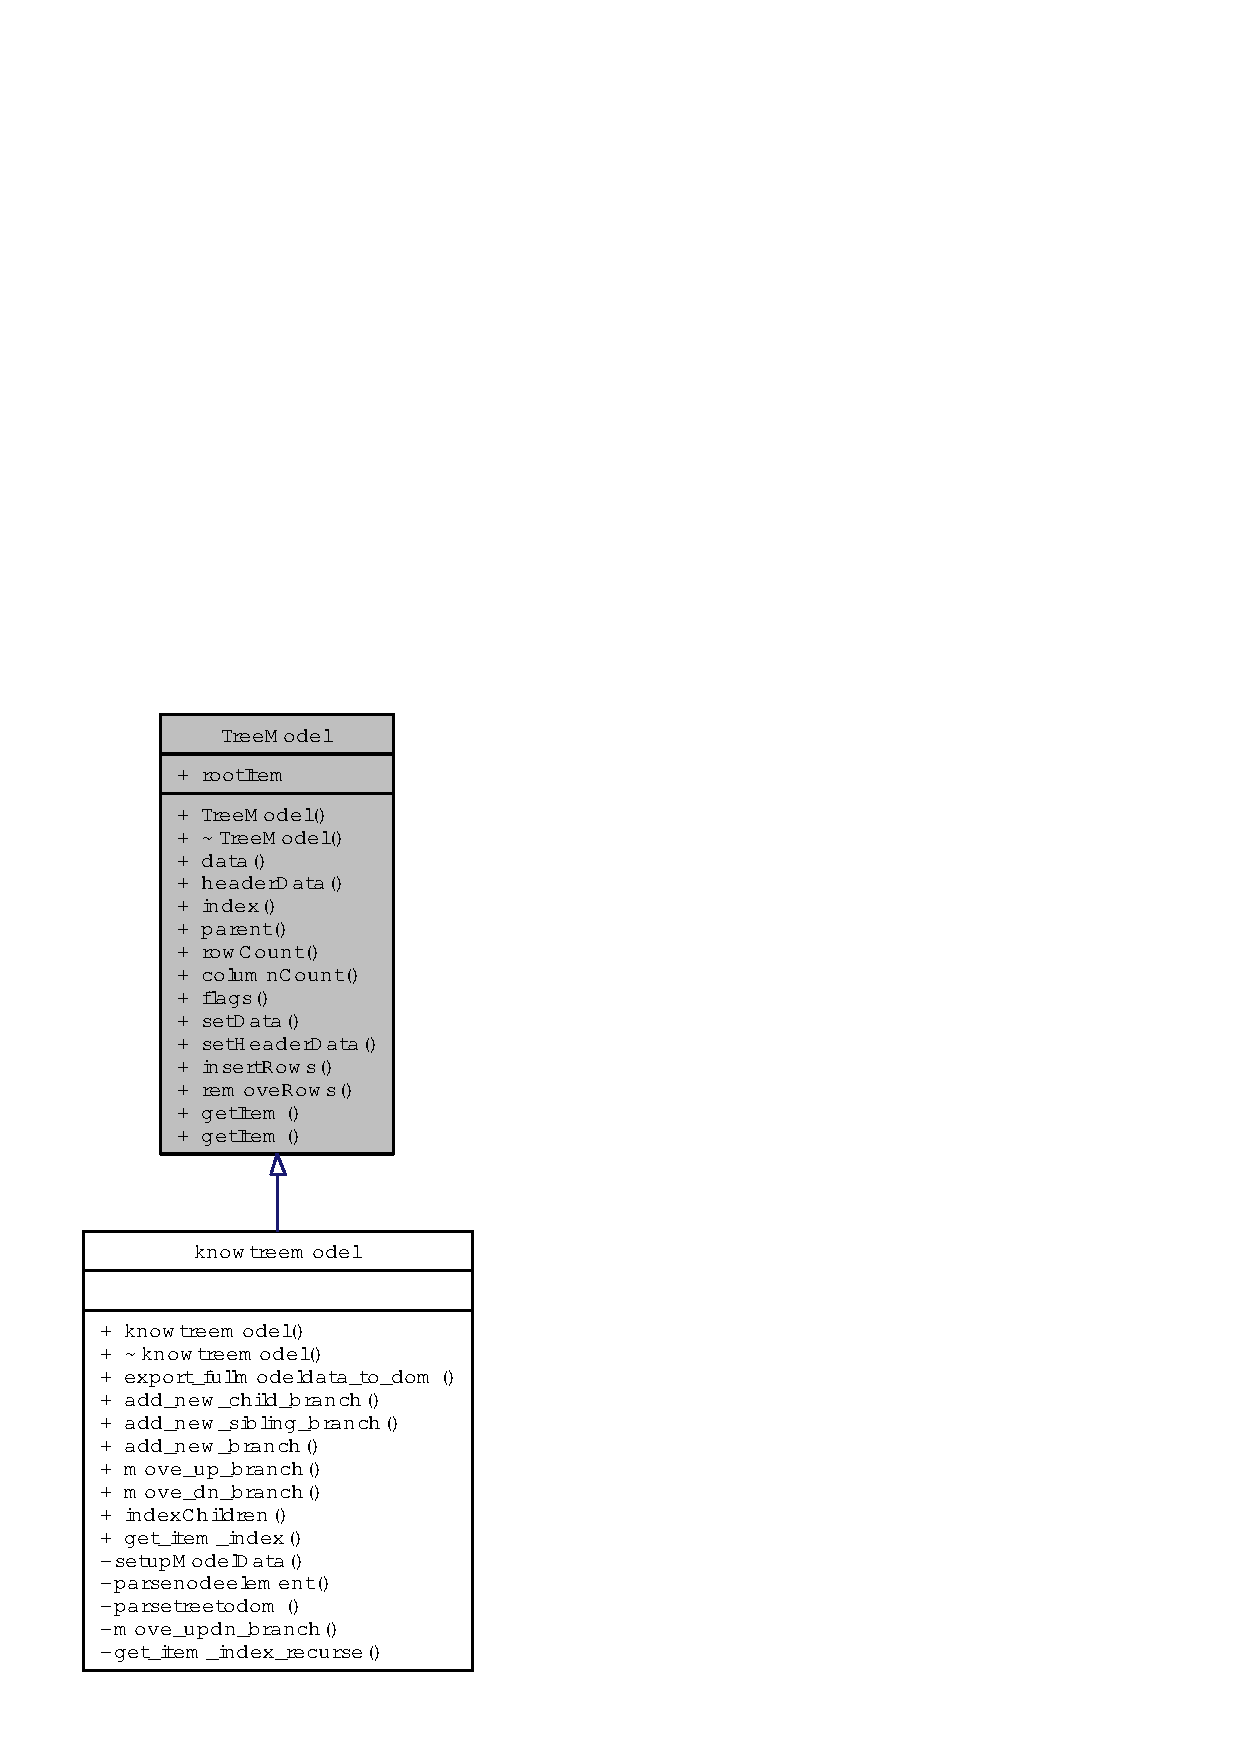
\includegraphics[width=115pt]{classTreeModel__inherit__graph}
\end{center}
\end{figure}
Collaboration diagram for Tree\-Model:\begin{figure}[H]
\begin{center}
\leavevmode
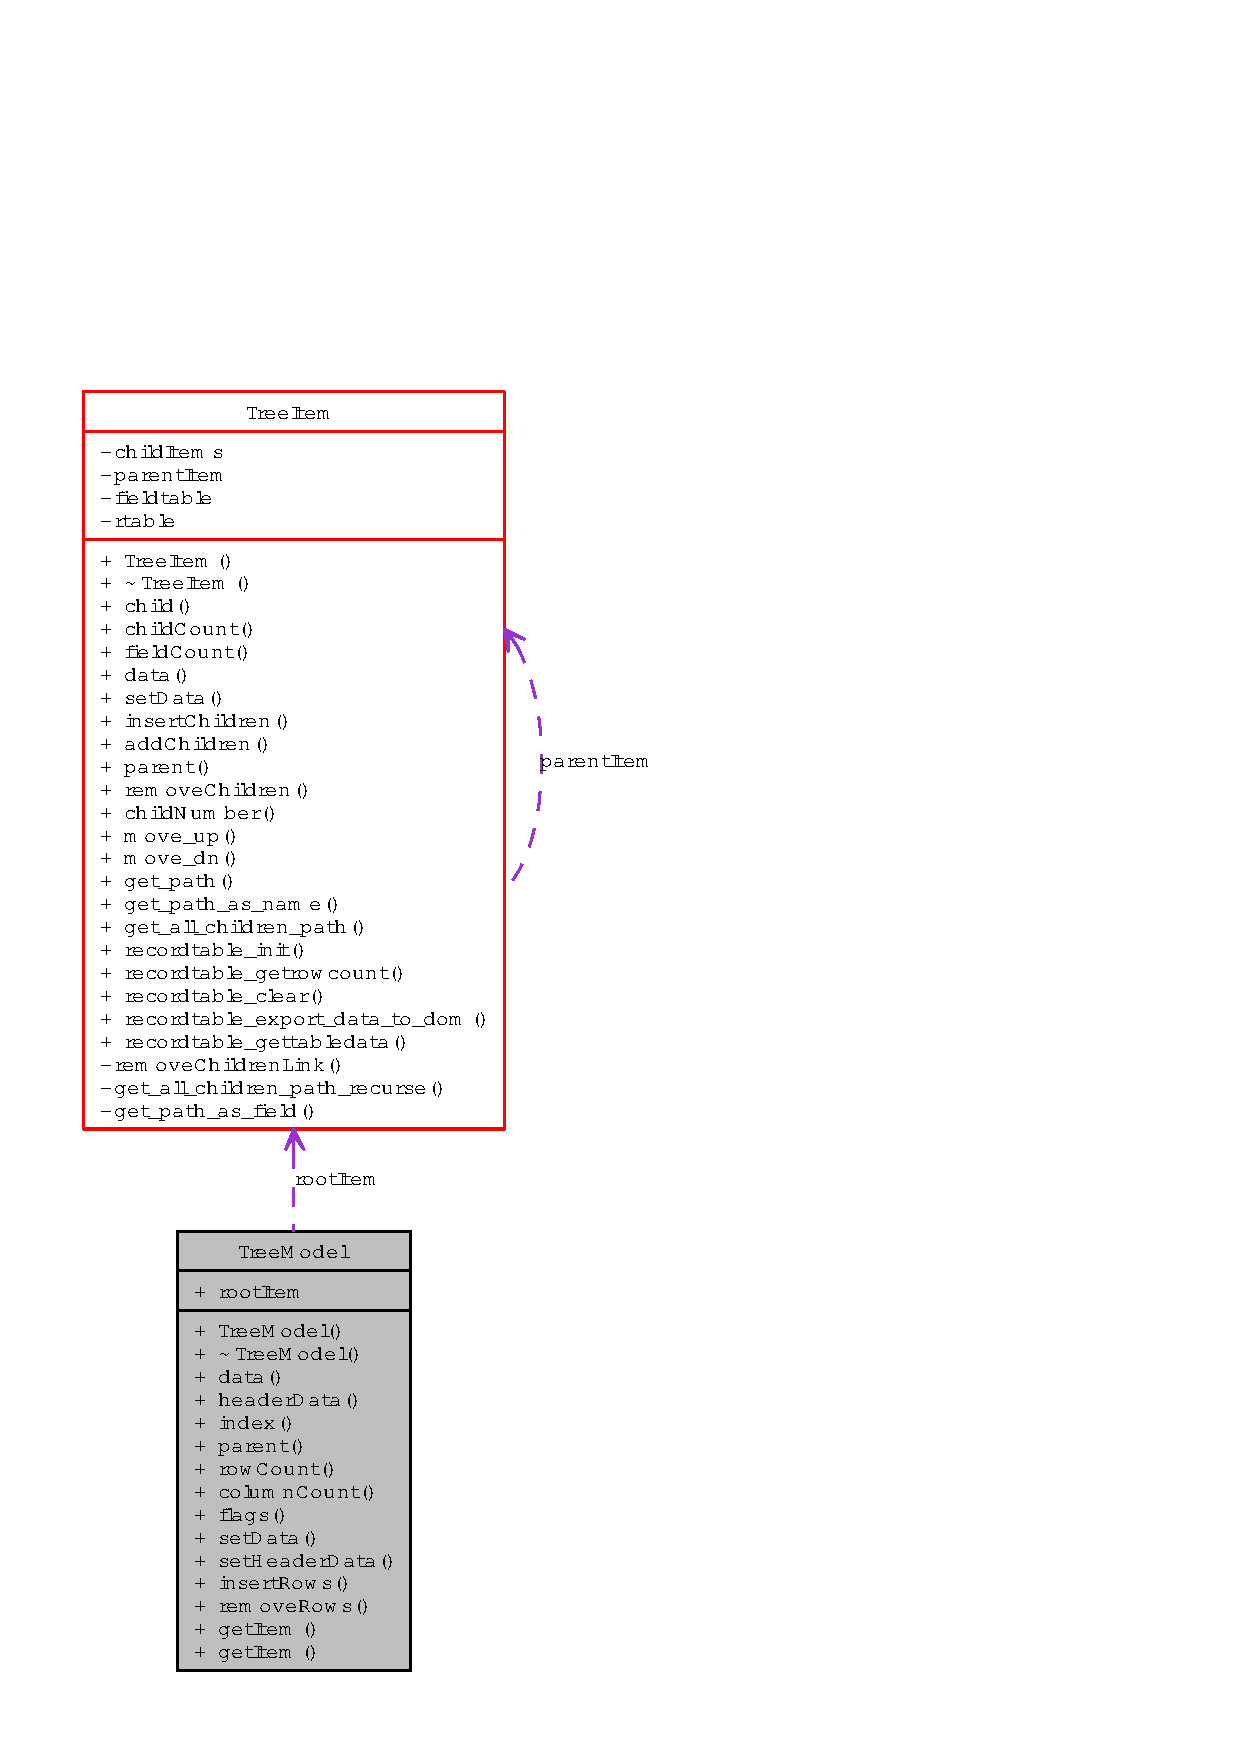
\includegraphics[width=160pt]{classTreeModel__coll__graph}
\end{center}
\end{figure}
\subsection*{Public Member Functions}
\begin{CompactItemize}
\item 
{\bf Tree\-Model} (QObject $\ast$parent=0)
\item 
{\bf $\sim$Tree\-Model} (void)
\item 
QVariant {\bf data} (const QModel\-Index \&index, int role) const
\item 
QVariant {\bf header\-Data} (int section, Qt::Orientation orientation, int role=Qt::Display\-Role) const
\item 
QModel\-Index {\bf index} (int row, int column, const QModel\-Index \&parent=QModel\-Index()) const
\item 
QModel\-Index {\bf parent} (const QModel\-Index \&index) const
\item 
int {\bf row\-Count} (const QModel\-Index \&parent=QModel\-Index()) const
\begin{CompactList}\small\item\em [8] \item\end{CompactList}\item 
int {\bf column\-Count} (const QModel\-Index \&parent=QModel\-Index()) const
\item 
Qt::Item\-Flags {\bf flags} (const QModel\-Index \&index) const
\item 
bool {\bf set\-Data} (const QModel\-Index \&index, const QVariant \&value, int role=Qt::Edit\-Role)
\item 
bool {\bf set\-Header\-Data} (int section, Qt::Orientation orientation, const QVariant \&value, int role=Qt::Edit\-Role)
\item 
bool {\bf insert\-Rows} (int position, int rows, const QModel\-Index \&parent=QModel\-Index())
\item 
bool {\bf remove\-Rows} (int position, int rows, const QModel\-Index \&parent=QModel\-Index())
\item 
{\bf Tree\-Item} $\ast$ {\bf get\-Item} (const QModel\-Index \&index) const
\item 
{\bf Tree\-Item} $\ast$ {\bf get\-Item} (QString\-List path) const
\end{CompactItemize}
\subsection*{Public Attributes}
\begin{CompactItemize}
\item 
{\bf Tree\-Item} $\ast$ {\bf root\-Item}
\end{CompactItemize}


\subsection{Detailed Description}




Definition at line 15 of file treemodel.h.

\subsection{Constructor \& Destructor Documentation}
\index{TreeModel@{Tree\-Model}!TreeModel@{TreeModel}}
\index{TreeModel@{TreeModel}!TreeModel@{Tree\-Model}}
\subsubsection{\setlength{\rightskip}{0pt plus 5cm}Tree\-Model::Tree\-Model (QObject $\ast$ {\em parent} = {\tt 0})}\label{classTreeModel_128d1d9d72775d1dfd3be4632c794ce3}




Definition at line 8 of file treemodel.cpp.\index{TreeModel@{Tree\-Model}!~TreeModel@{$\sim$TreeModel}}
\index{~TreeModel@{$\sim$TreeModel}!TreeModel@{Tree\-Model}}
\subsubsection{\setlength{\rightskip}{0pt plus 5cm}Tree\-Model::$\sim$Tree\-Model (void)}\label{classTreeModel_b200d2353bb3901d55ee3fab9d70d3ab}




Definition at line 13 of file treemodel.cpp.

\subsection{Member Function Documentation}
\index{TreeModel@{Tree\-Model}!data@{data}}
\index{data@{data}!TreeModel@{Tree\-Model}}
\subsubsection{\setlength{\rightskip}{0pt plus 5cm}QVariant Tree\-Model::data (const QModel\-Index \& {\em index}, int {\em role}) const}\label{classTreeModel_986b92267ac9cdc90519c10404192bbd}




Definition at line 29 of file treemodel.cpp.

References Tree\-Item::data(), get\-Item(), and Tree\-Item::recordtable\_\-getrowcount().

Referenced by get\-Item().

Here is the call graph for this function:\begin{figure}[H]
\begin{center}
\leavevmode
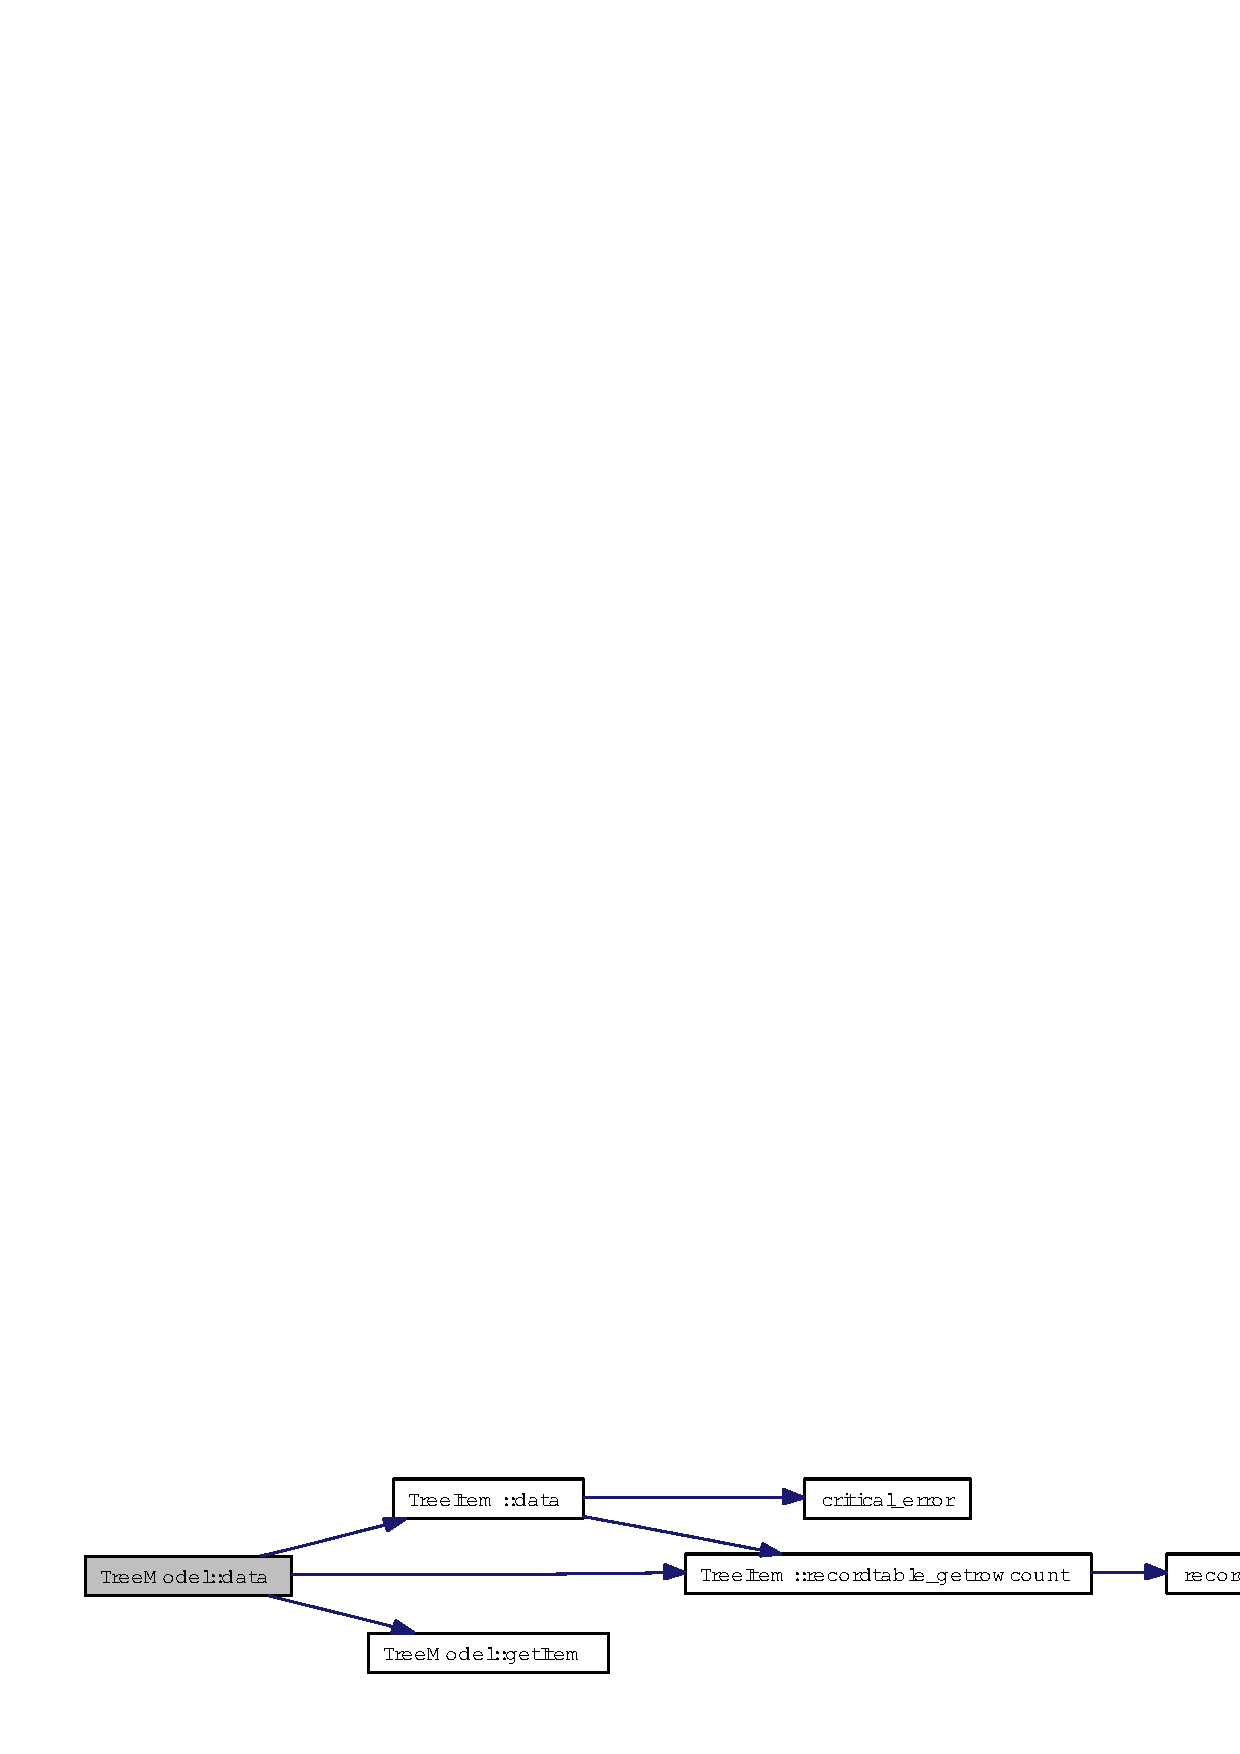
\includegraphics[width=344pt]{classTreeModel_986b92267ac9cdc90519c10404192bbd_cgraph}
\end{center}
\end{figure}


Here is the caller graph for this function:\begin{figure}[H]
\begin{center}
\leavevmode
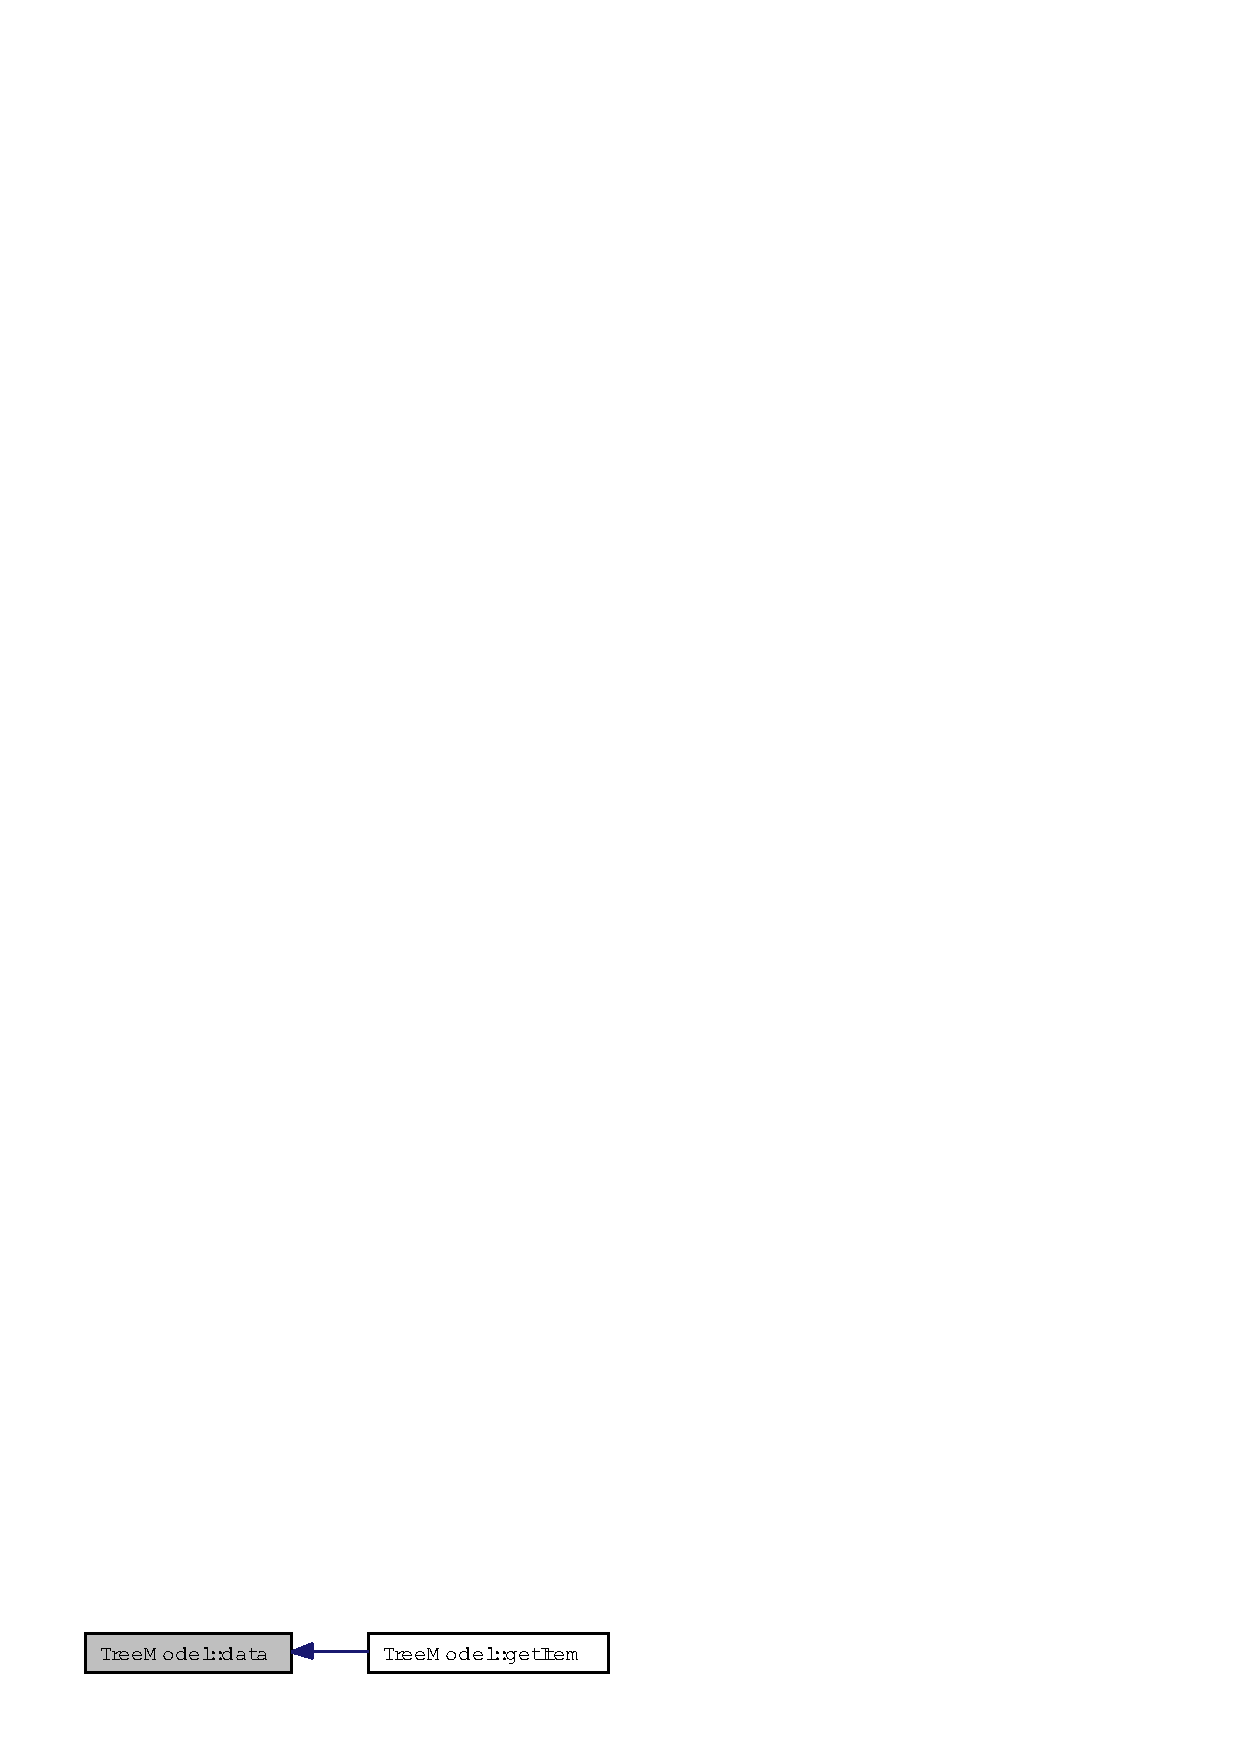
\includegraphics[width=148pt]{classTreeModel_986b92267ac9cdc90519c10404192bbd_icgraph}
\end{center}
\end{figure}
\index{TreeModel@{Tree\-Model}!headerData@{headerData}}
\index{headerData@{headerData}!TreeModel@{Tree\-Model}}
\subsubsection{\setlength{\rightskip}{0pt plus 5cm}QVariant Tree\-Model::header\-Data (int {\em section}, Qt::Orientation {\em orientation}, int {\em role} = {\tt Qt::DisplayRole}) const}\label{classTreeModel_59b8e296fb38595cd5459aa75dd507ba}




Definition at line 112 of file treemodel.cpp.\index{TreeModel@{Tree\-Model}!index@{index}}
\index{index@{index}!TreeModel@{Tree\-Model}}
\subsubsection{\setlength{\rightskip}{0pt plus 5cm}QModel\-Index Tree\-Model::index (int {\em row}, int {\em column}, const QModel\-Index \& {\em parent} = {\tt QModelIndex()}) const}\label{classTreeModel_0e6e6bbdb55d08be64cab7bafba2ce21}




Definition at line 135 of file treemodel.cpp.

References Tree\-Item::child(), and get\-Item().

Referenced by knowtreemodel::index\-Children(), treescreen::ins\_\-branch(), and knowtreemodel::move\_\-updn\_\-branch().

Here is the call graph for this function:\begin{figure}[H]
\begin{center}
\leavevmode
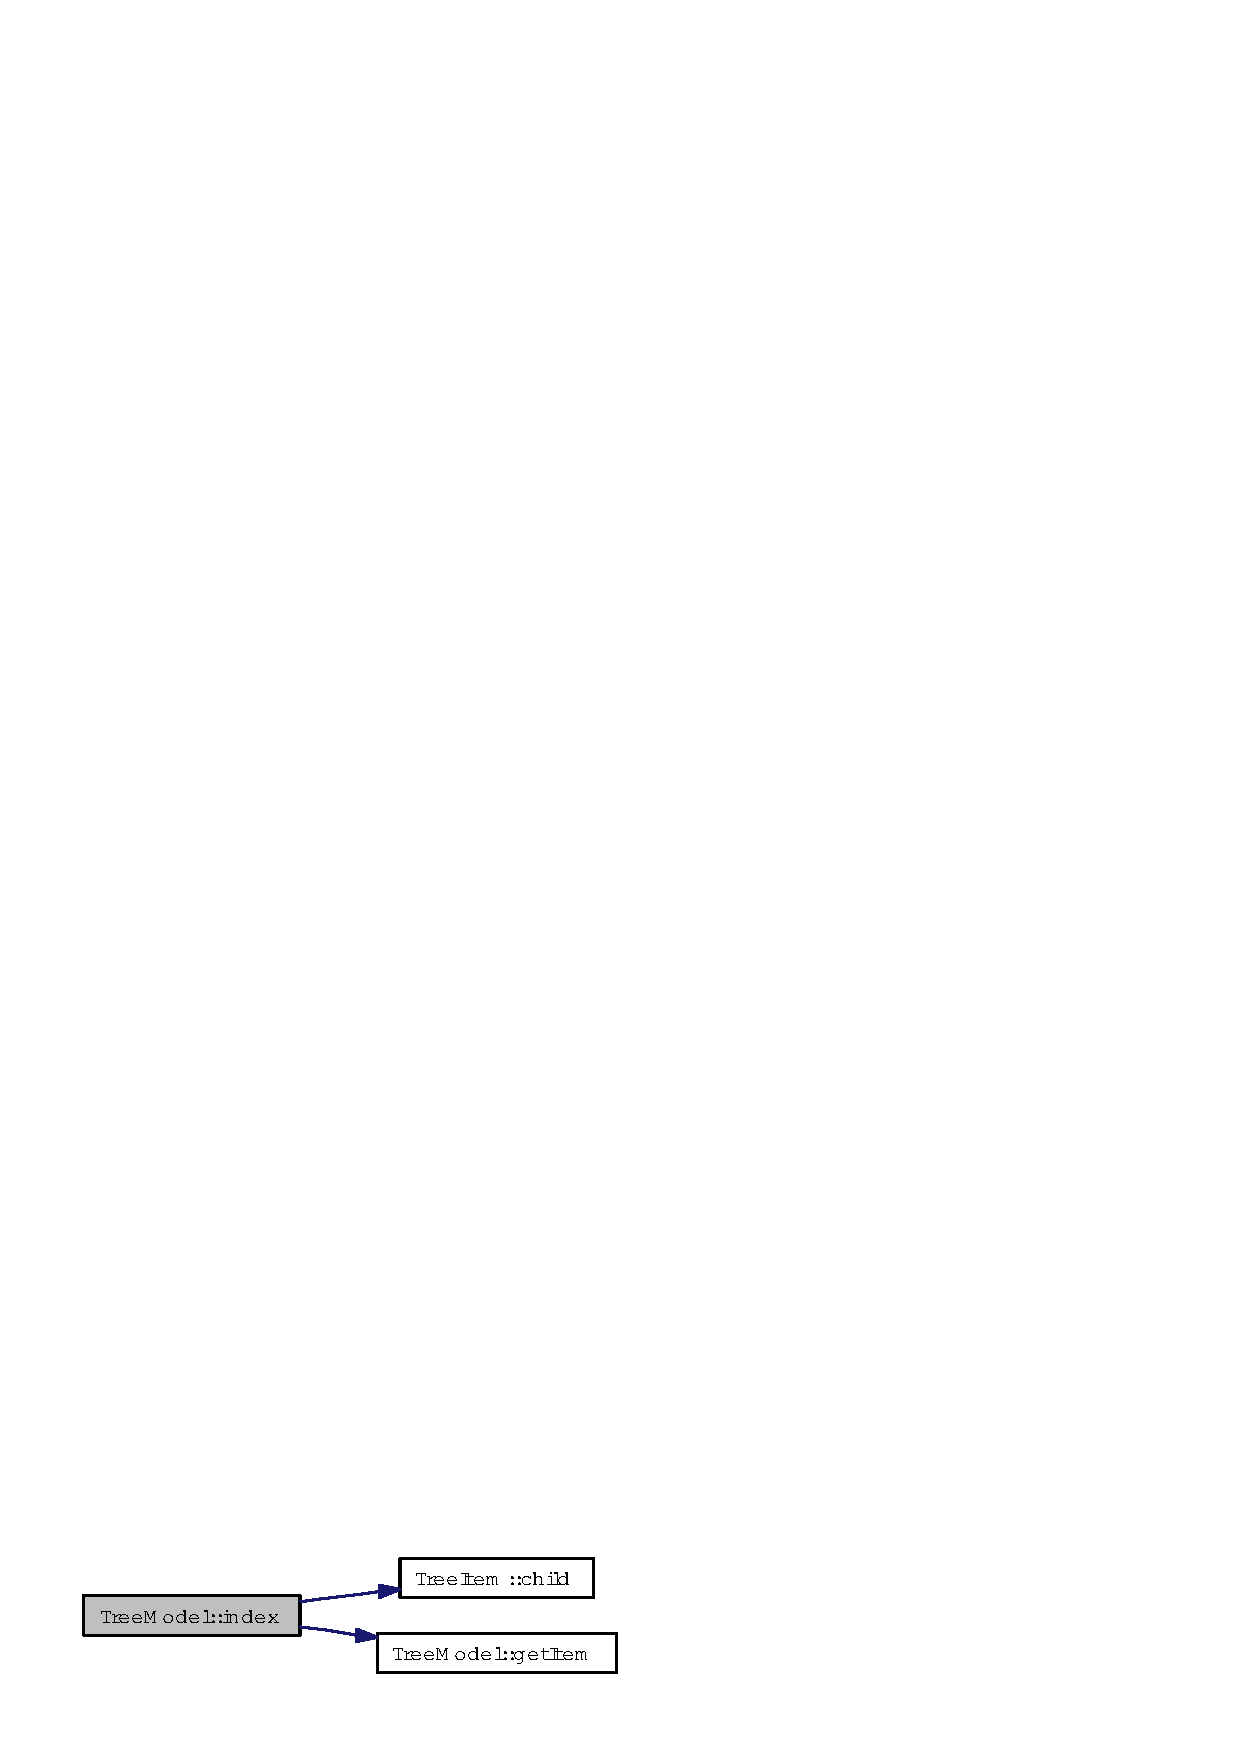
\includegraphics[width=150pt]{classTreeModel_0e6e6bbdb55d08be64cab7bafba2ce21_cgraph}
\end{center}
\end{figure}


Here is the caller graph for this function:\begin{figure}[H]
\begin{center}
\leavevmode
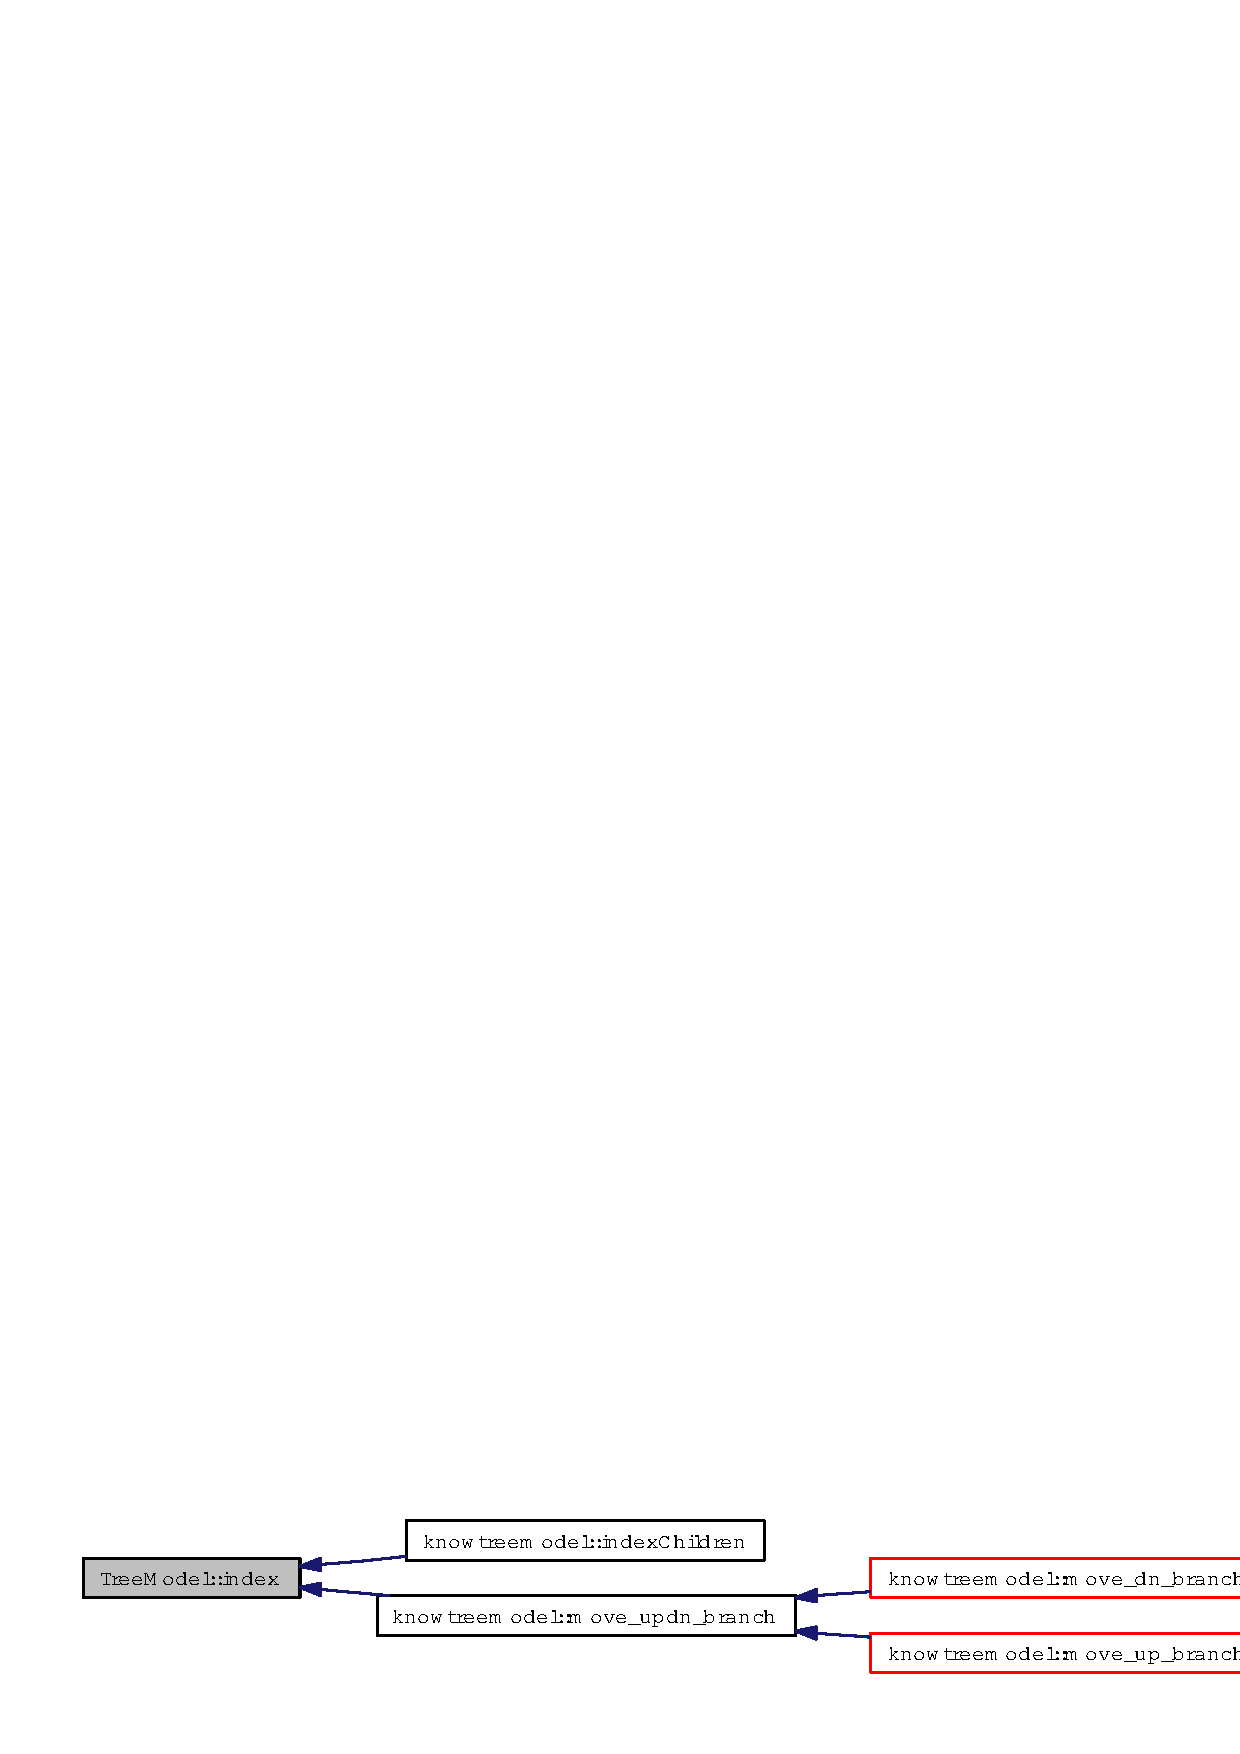
\includegraphics[width=305pt]{classTreeModel_0e6e6bbdb55d08be64cab7bafba2ce21_icgraph}
\end{center}
\end{figure}
\index{TreeModel@{Tree\-Model}!parent@{parent}}
\index{parent@{parent}!TreeModel@{Tree\-Model}}
\subsubsection{\setlength{\rightskip}{0pt plus 5cm}QModel\-Index Tree\-Model::parent (const QModel\-Index \& {\em index}) const}\label{classTreeModel_d29cef85c6bb0db25fb3d5b844c22e94}




Definition at line 168 of file treemodel.cpp.

References Tree\-Item::child\-Number(), get\-Item(), Tree\-Item::parent(), and root\-Item.

Referenced by knowtreemodel::add\_\-new\_\-branch(), knowtreemodel::add\_\-new\_\-child\_\-branch(), knowtreemodel::add\_\-new\_\-sibling\_\-branch(), knowtreemodel::parsenodeelement(), and knowtreemodel::setup\-Model\-Data().

Here is the call graph for this function:\begin{figure}[H]
\begin{center}
\leavevmode
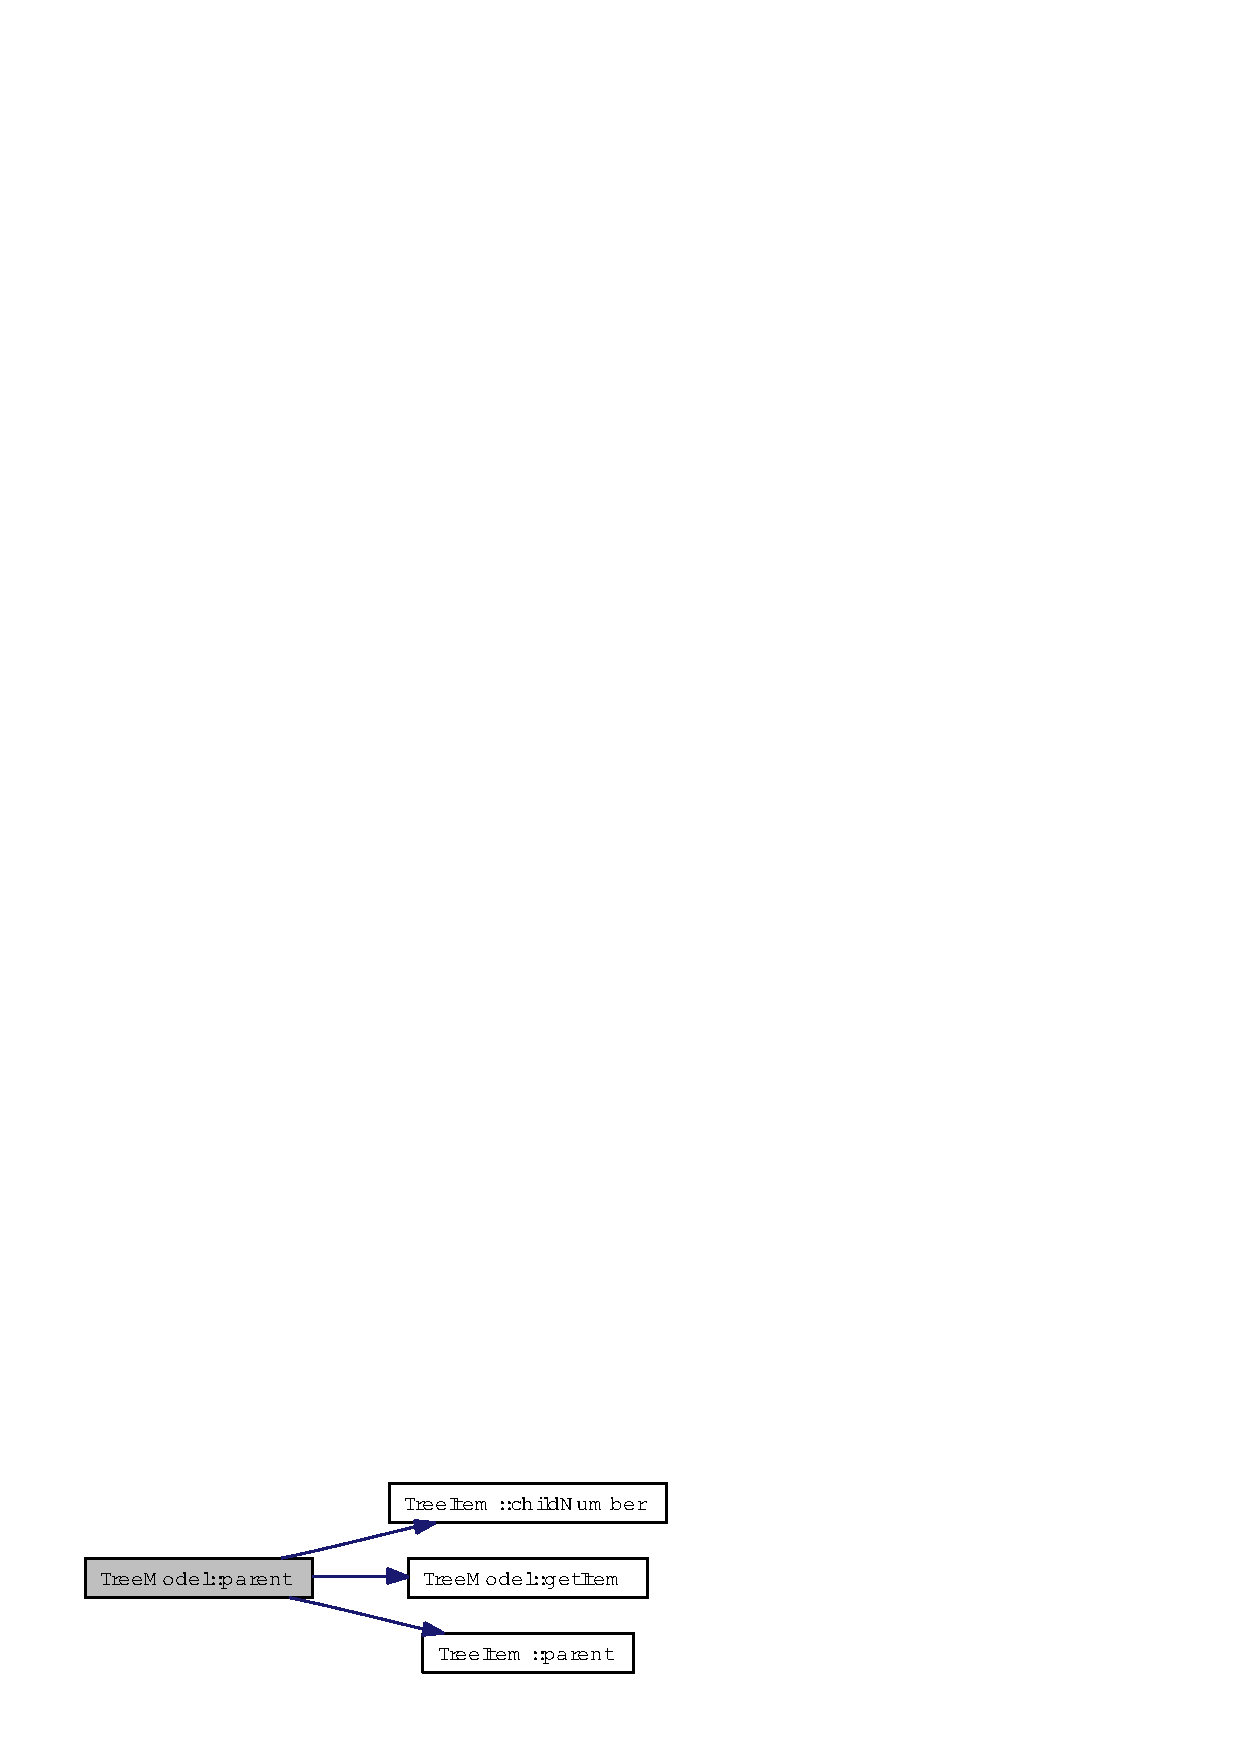
\includegraphics[width=162pt]{classTreeModel_d29cef85c6bb0db25fb3d5b844c22e94_cgraph}
\end{center}
\end{figure}


Here is the caller graph for this function:\begin{figure}[H]
\begin{center}
\leavevmode
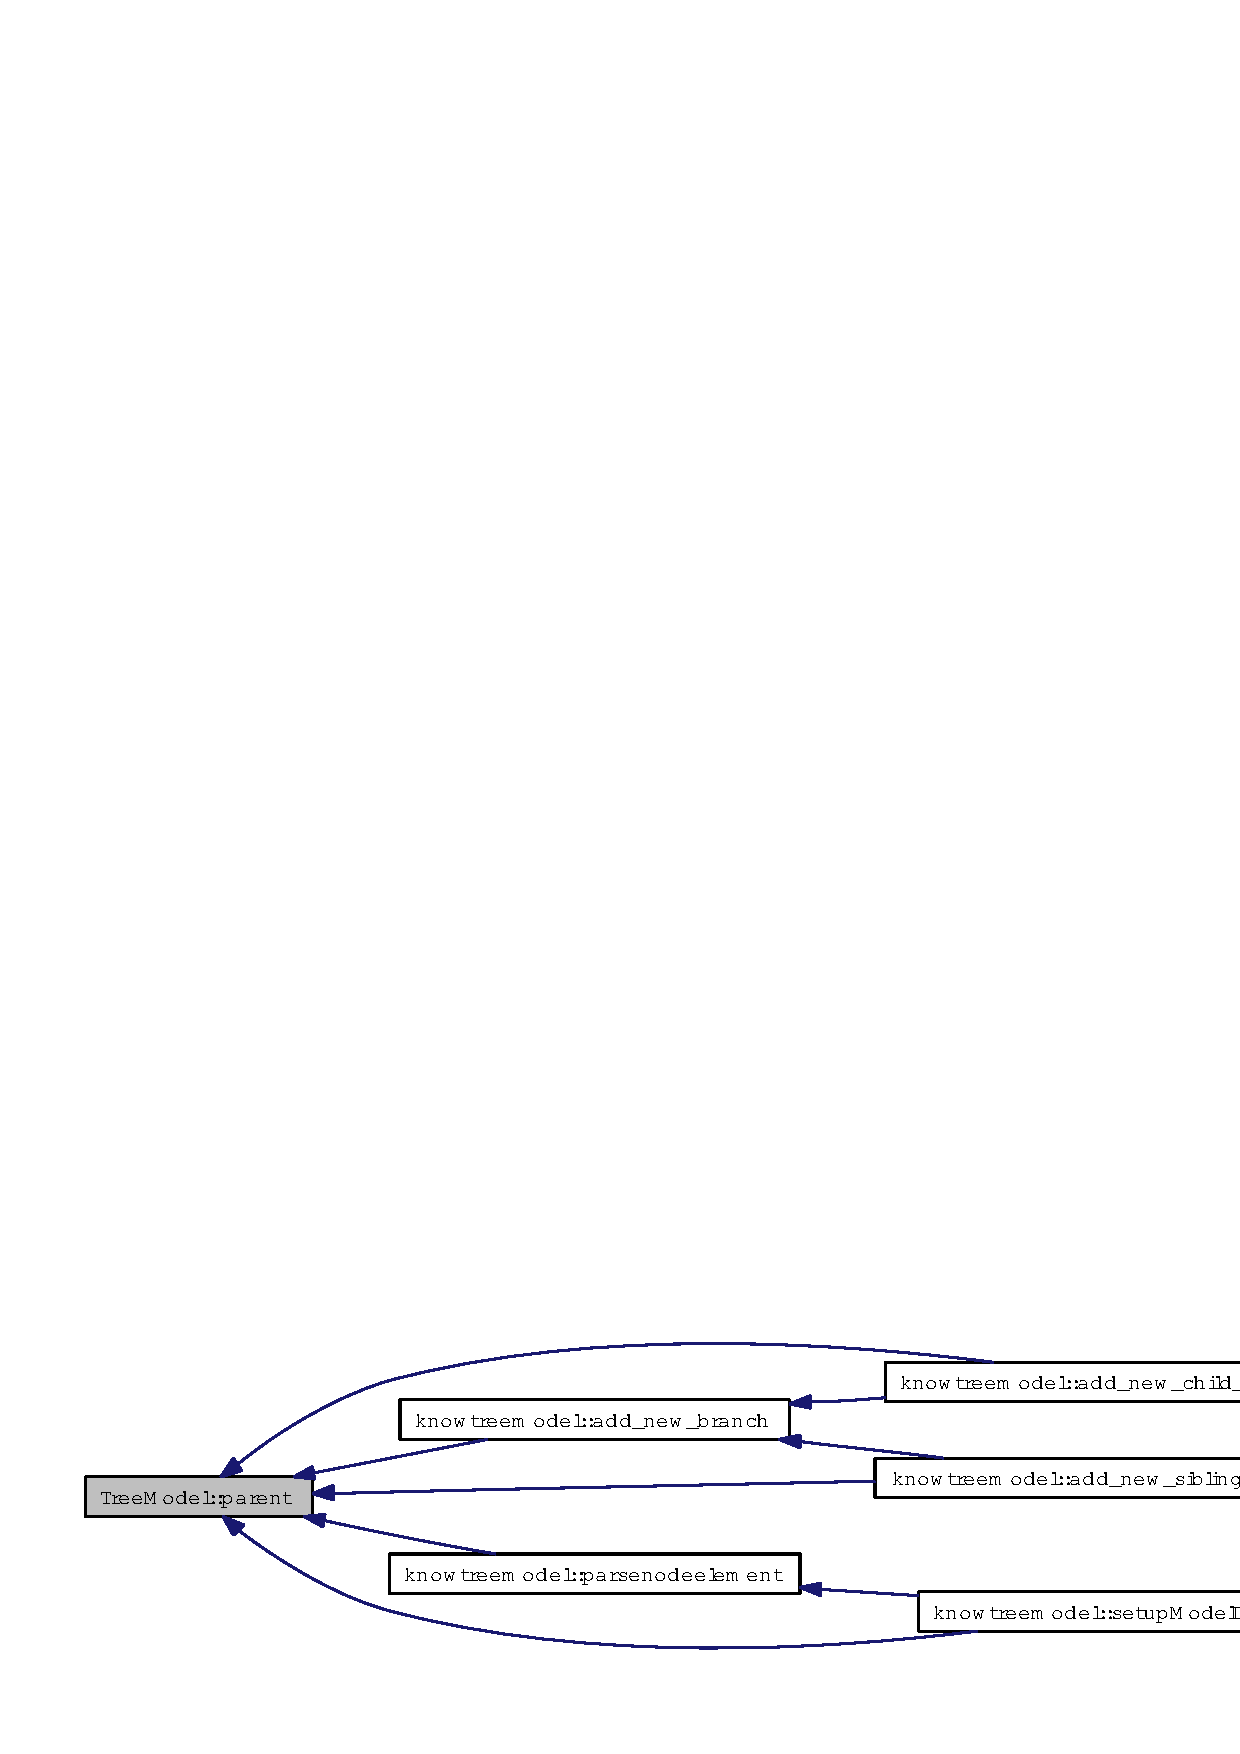
\includegraphics[width=325pt]{classTreeModel_d29cef85c6bb0db25fb3d5b844c22e94_icgraph}
\end{center}
\end{figure}
\index{TreeModel@{Tree\-Model}!rowCount@{rowCount}}
\index{rowCount@{rowCount}!TreeModel@{Tree\-Model}}
\subsubsection{\setlength{\rightskip}{0pt plus 5cm}int Tree\-Model::row\-Count (const QModel\-Index \& {\em parent} = {\tt QModelIndex()}) const}\label{classTreeModel_a741dd31a085f8a2495fc1d7feb50226}


[8] 



Definition at line 196 of file treemodel.cpp.

References Tree\-Item::child\-Count(), and get\-Item().

Here is the call graph for this function:\begin{figure}[H]
\begin{center}
\leavevmode
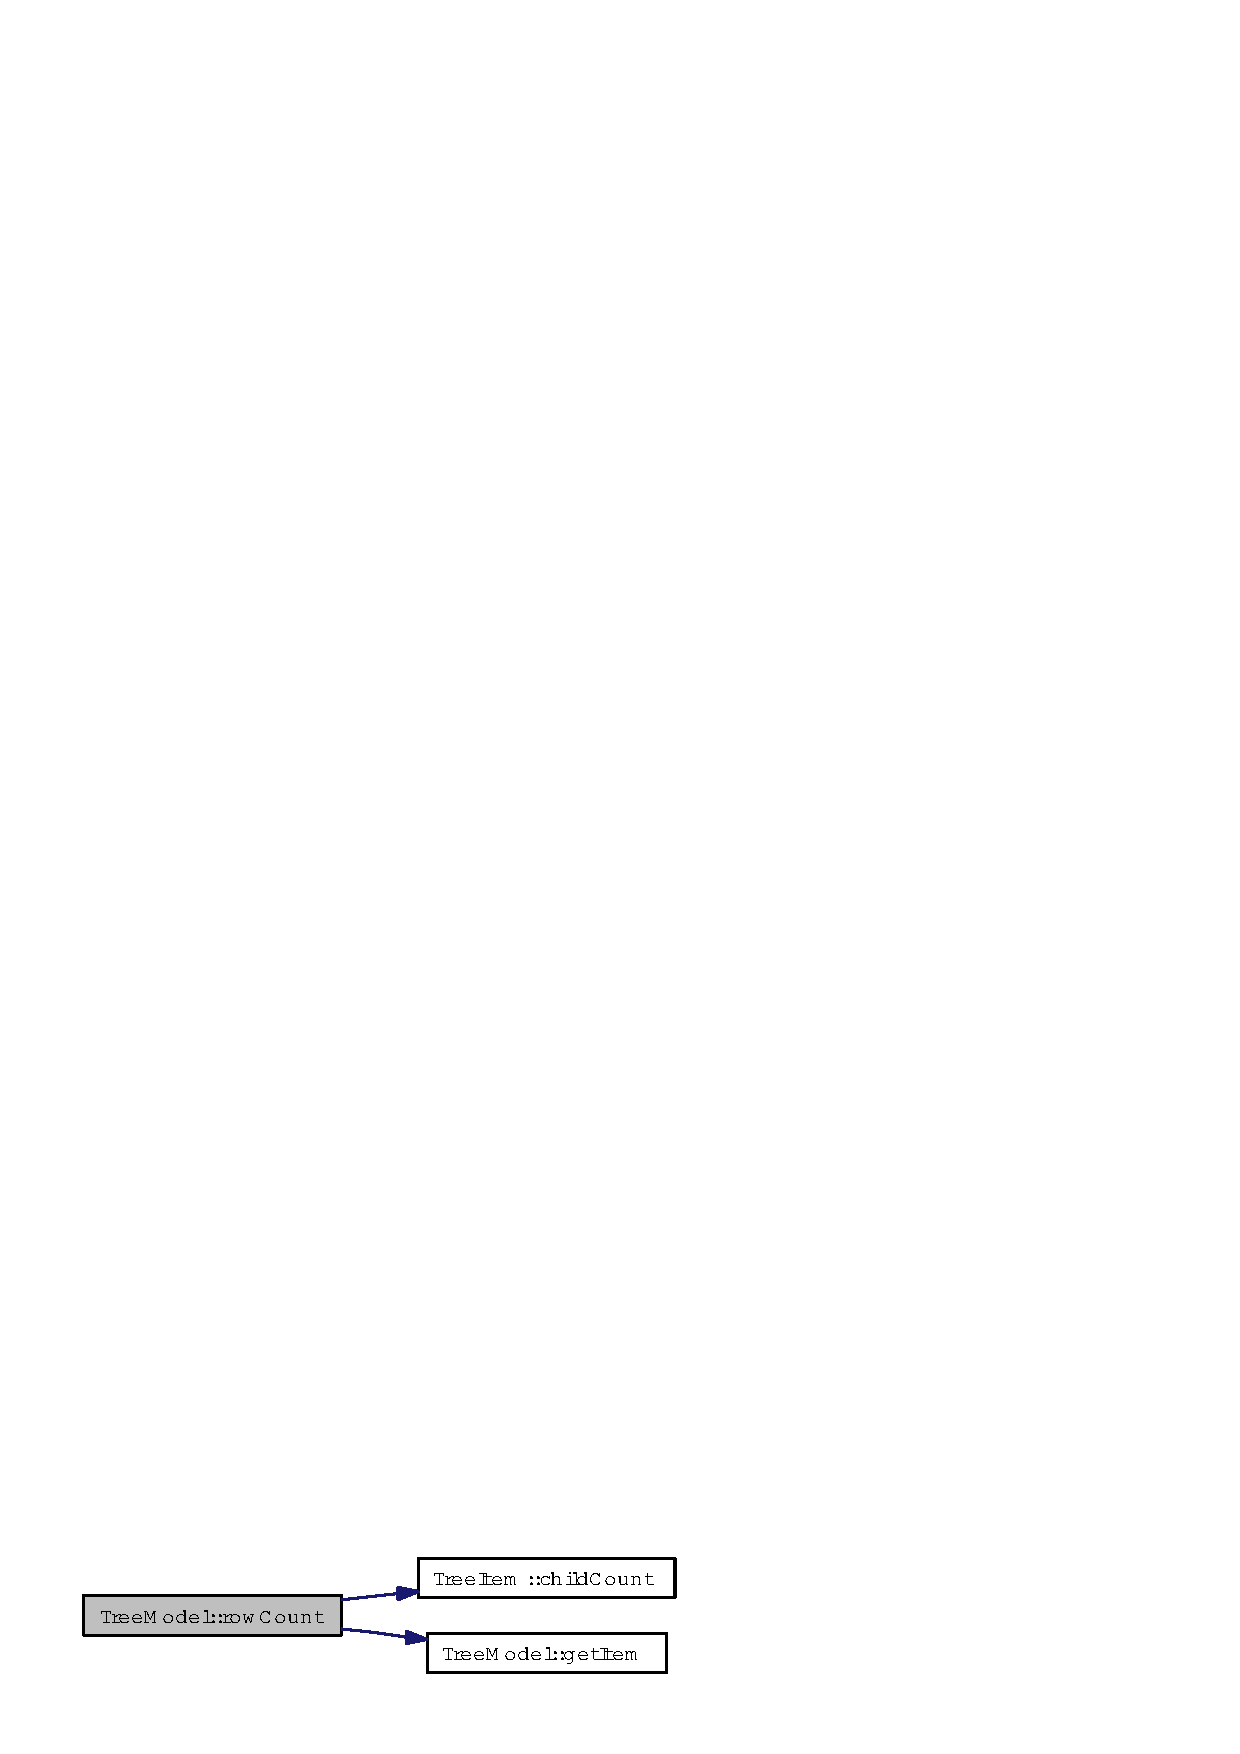
\includegraphics[width=164pt]{classTreeModel_a741dd31a085f8a2495fc1d7feb50226_cgraph}
\end{center}
\end{figure}
\index{TreeModel@{Tree\-Model}!columnCount@{columnCount}}
\index{columnCount@{columnCount}!TreeModel@{Tree\-Model}}
\subsubsection{\setlength{\rightskip}{0pt plus 5cm}int Tree\-Model::column\-Count (const QModel\-Index \& {\em parent} = {\tt QModelIndex()}) const}\label{classTreeModel_7c23a1d2d39fb76e3d28aa9a0a6f365a}




Definition at line 18 of file treemodel.cpp.\index{TreeModel@{Tree\-Model}!flags@{flags}}
\index{flags@{flags}!TreeModel@{Tree\-Model}}
\subsubsection{\setlength{\rightskip}{0pt plus 5cm}Qt::Item\-Flags Tree\-Model::flags (const QModel\-Index \& {\em index}) const}\label{classTreeModel_2f793c5b11ec3c46571e4598ee2398e7}




Definition at line 58 of file treemodel.cpp.\index{TreeModel@{Tree\-Model}!setData@{setData}}
\index{setData@{setData}!TreeModel@{Tree\-Model}}
\subsubsection{\setlength{\rightskip}{0pt plus 5cm}bool Tree\-Model::set\-Data (const QModel\-Index \& {\em index}, const QVariant \& {\em value}, int {\em role} = {\tt Qt::EditRole})}\label{classTreeModel_cd3341eaa58b720ea4e6d6a415145dbd}




Definition at line 205 of file treemodel.cpp.

References get\-Item(), and Tree\-Item::set\-Data().

Referenced by knowtreemodel::add\_\-new\_\-branch(), and knowtreemodel::parsenodeelement().

Here is the call graph for this function:\begin{figure}[H]
\begin{center}
\leavevmode
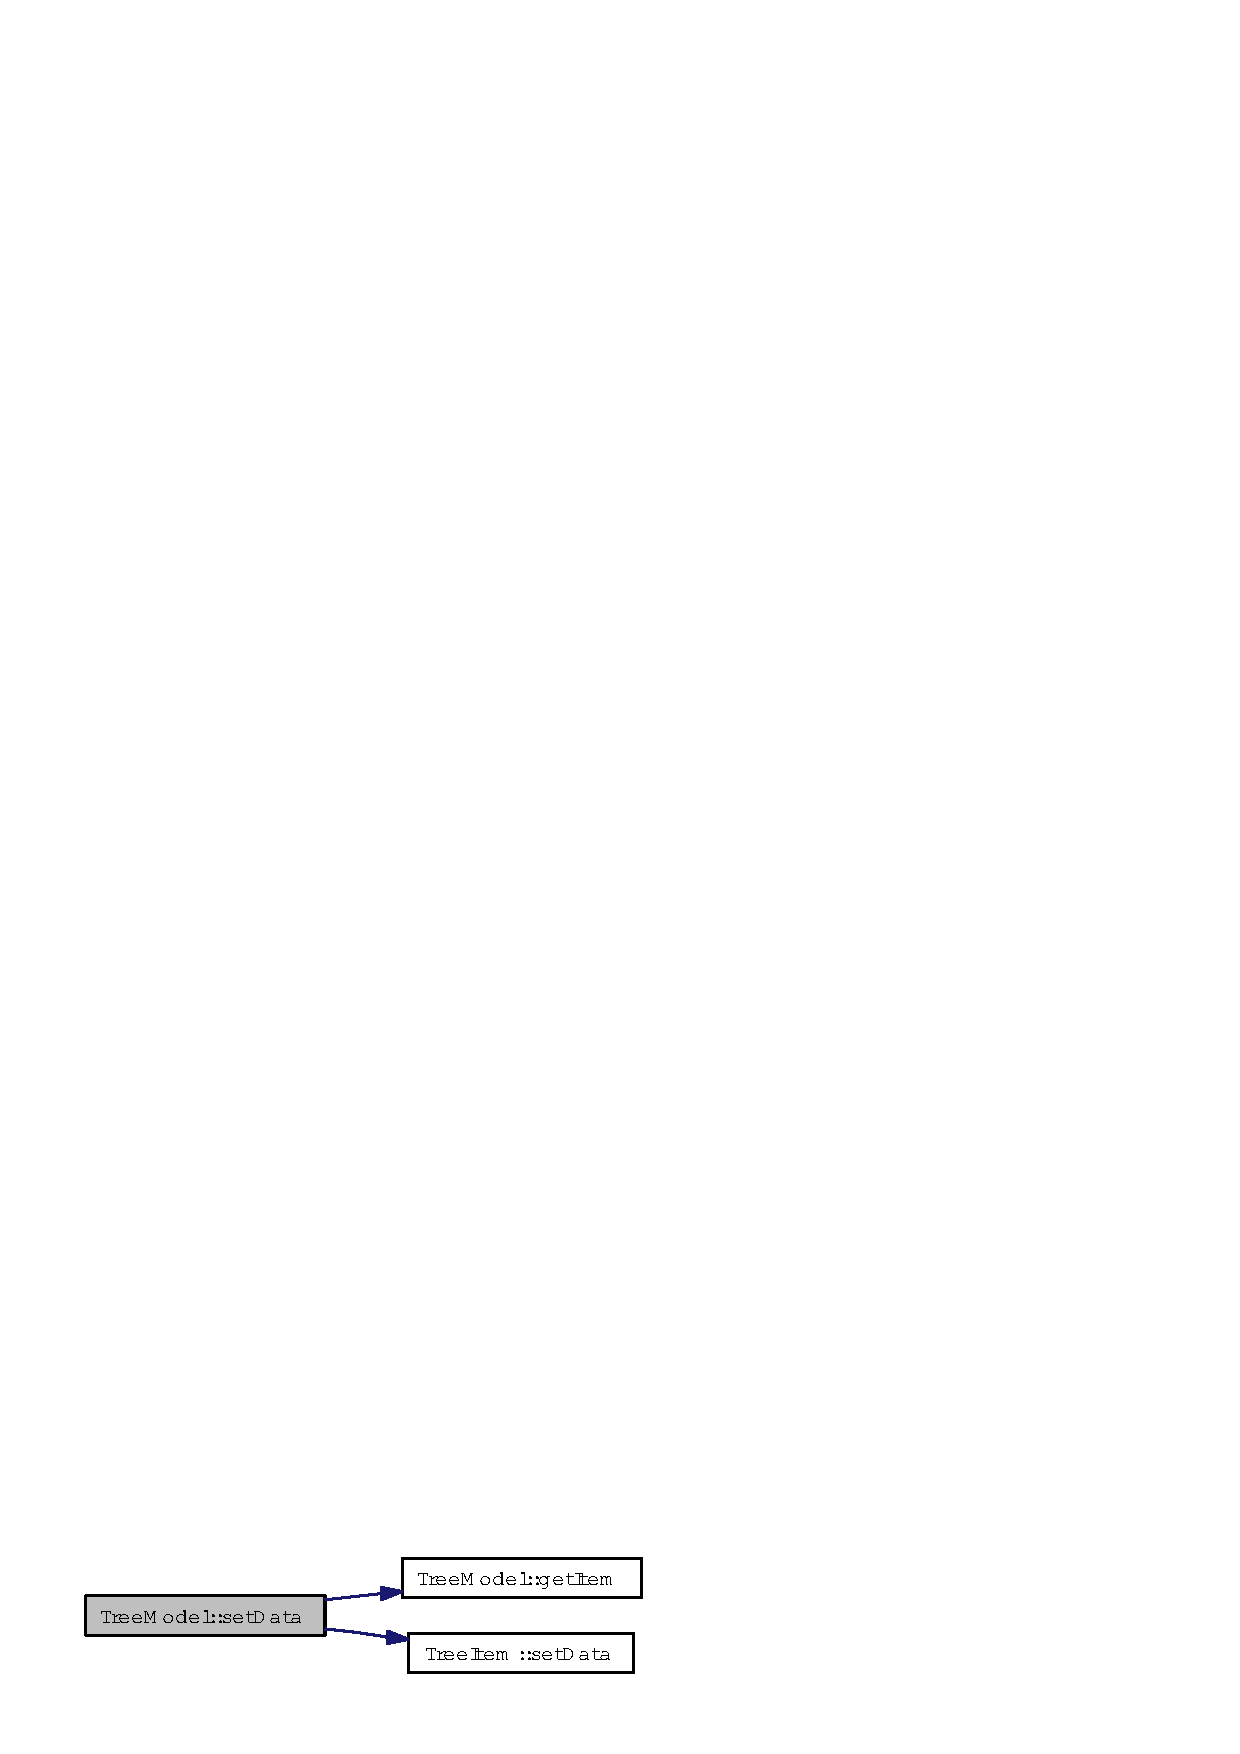
\includegraphics[width=156pt]{classTreeModel_cd3341eaa58b720ea4e6d6a415145dbd_cgraph}
\end{center}
\end{figure}


Here is the caller graph for this function:\begin{figure}[H]
\begin{center}
\leavevmode
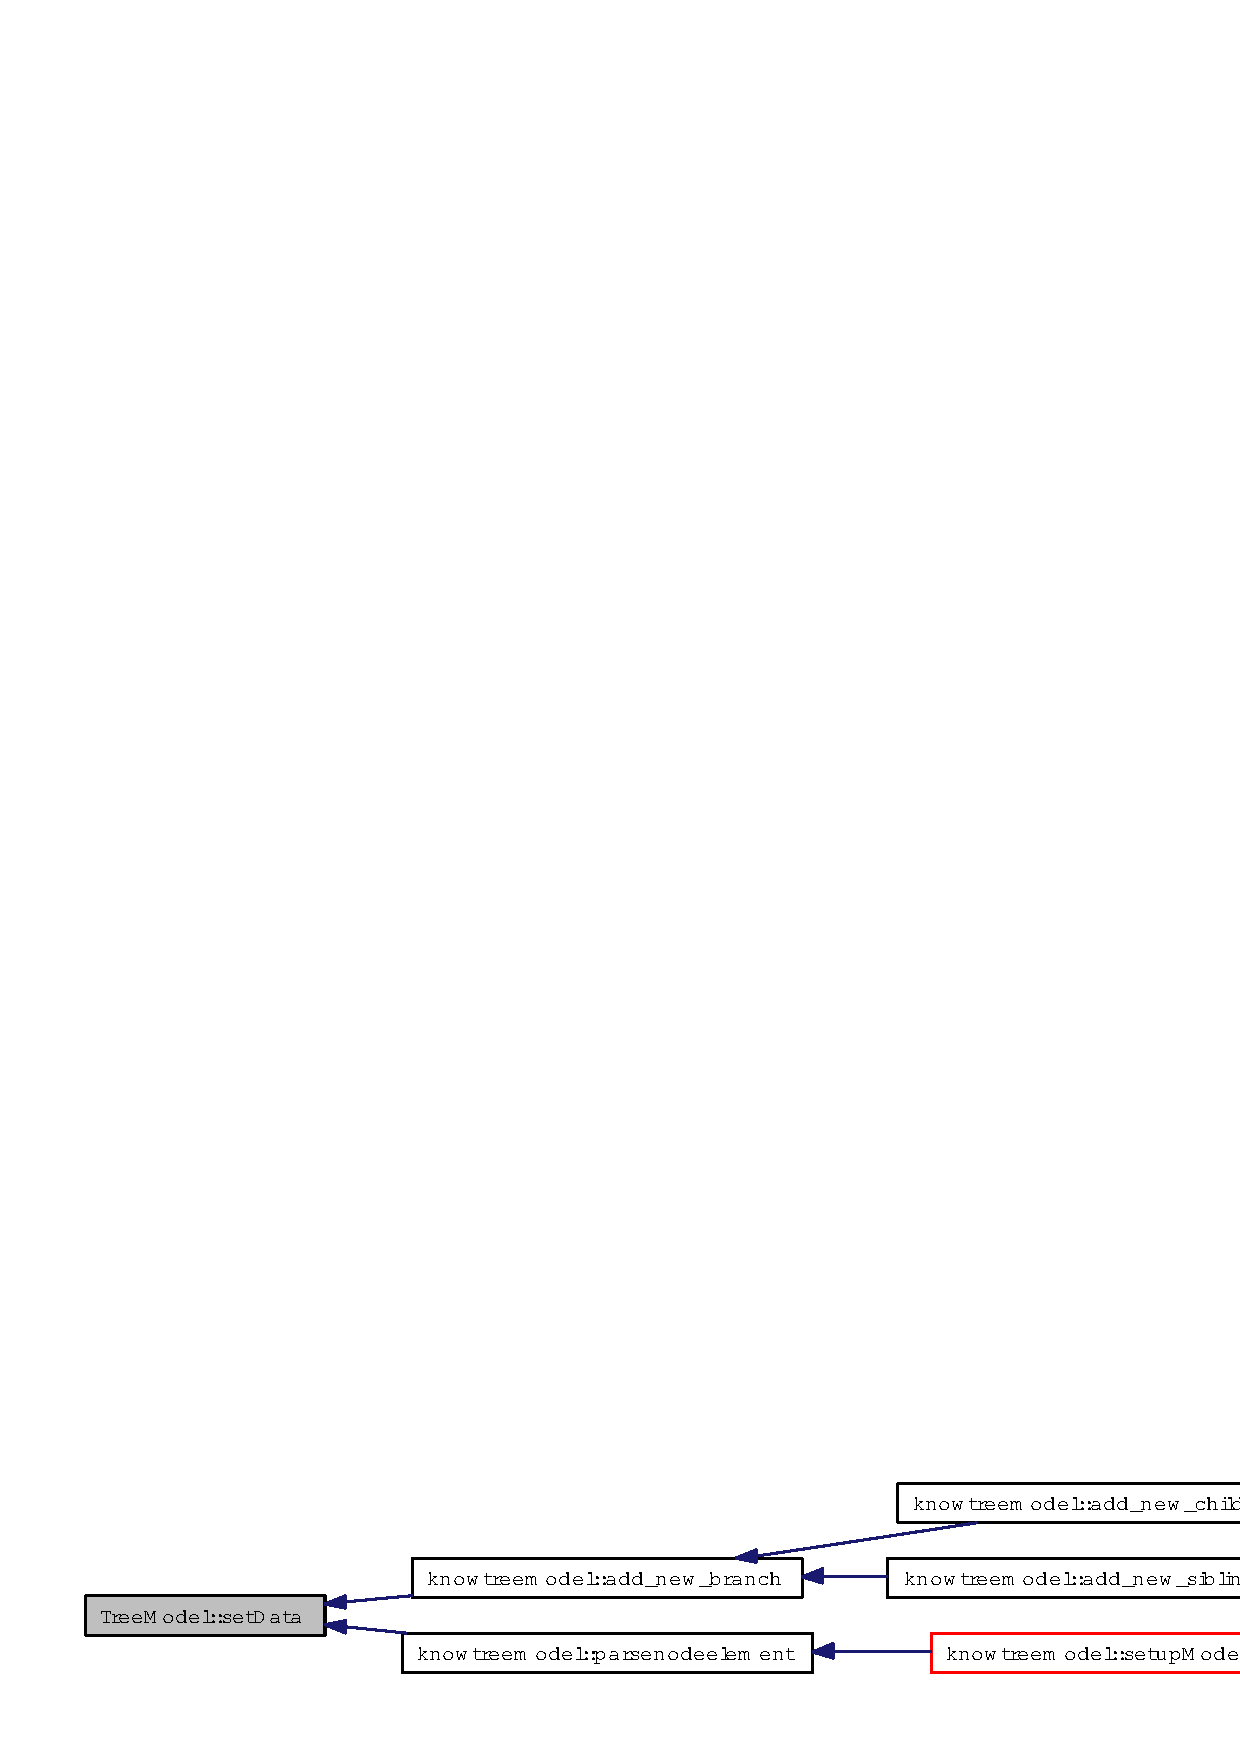
\includegraphics[width=328pt]{classTreeModel_cd3341eaa58b720ea4e6d6a415145dbd_icgraph}
\end{center}
\end{figure}
\index{TreeModel@{Tree\-Model}!setHeaderData@{setHeaderData}}
\index{setHeaderData@{setHeaderData}!TreeModel@{Tree\-Model}}
\subsubsection{\setlength{\rightskip}{0pt plus 5cm}bool Tree\-Model::set\-Header\-Data (int {\em section}, Qt::Orientation {\em orientation}, const QVariant \& {\em value}, int {\em role} = {\tt Qt::EditRole})}\label{classTreeModel_8d42cbbd50936e26241fb6a71ee9fb84}




Definition at line 219 of file treemodel.cpp.

References root\-Item, and Tree\-Item::set\-Data().

Here is the call graph for this function:\begin{figure}[H]
\begin{center}
\leavevmode
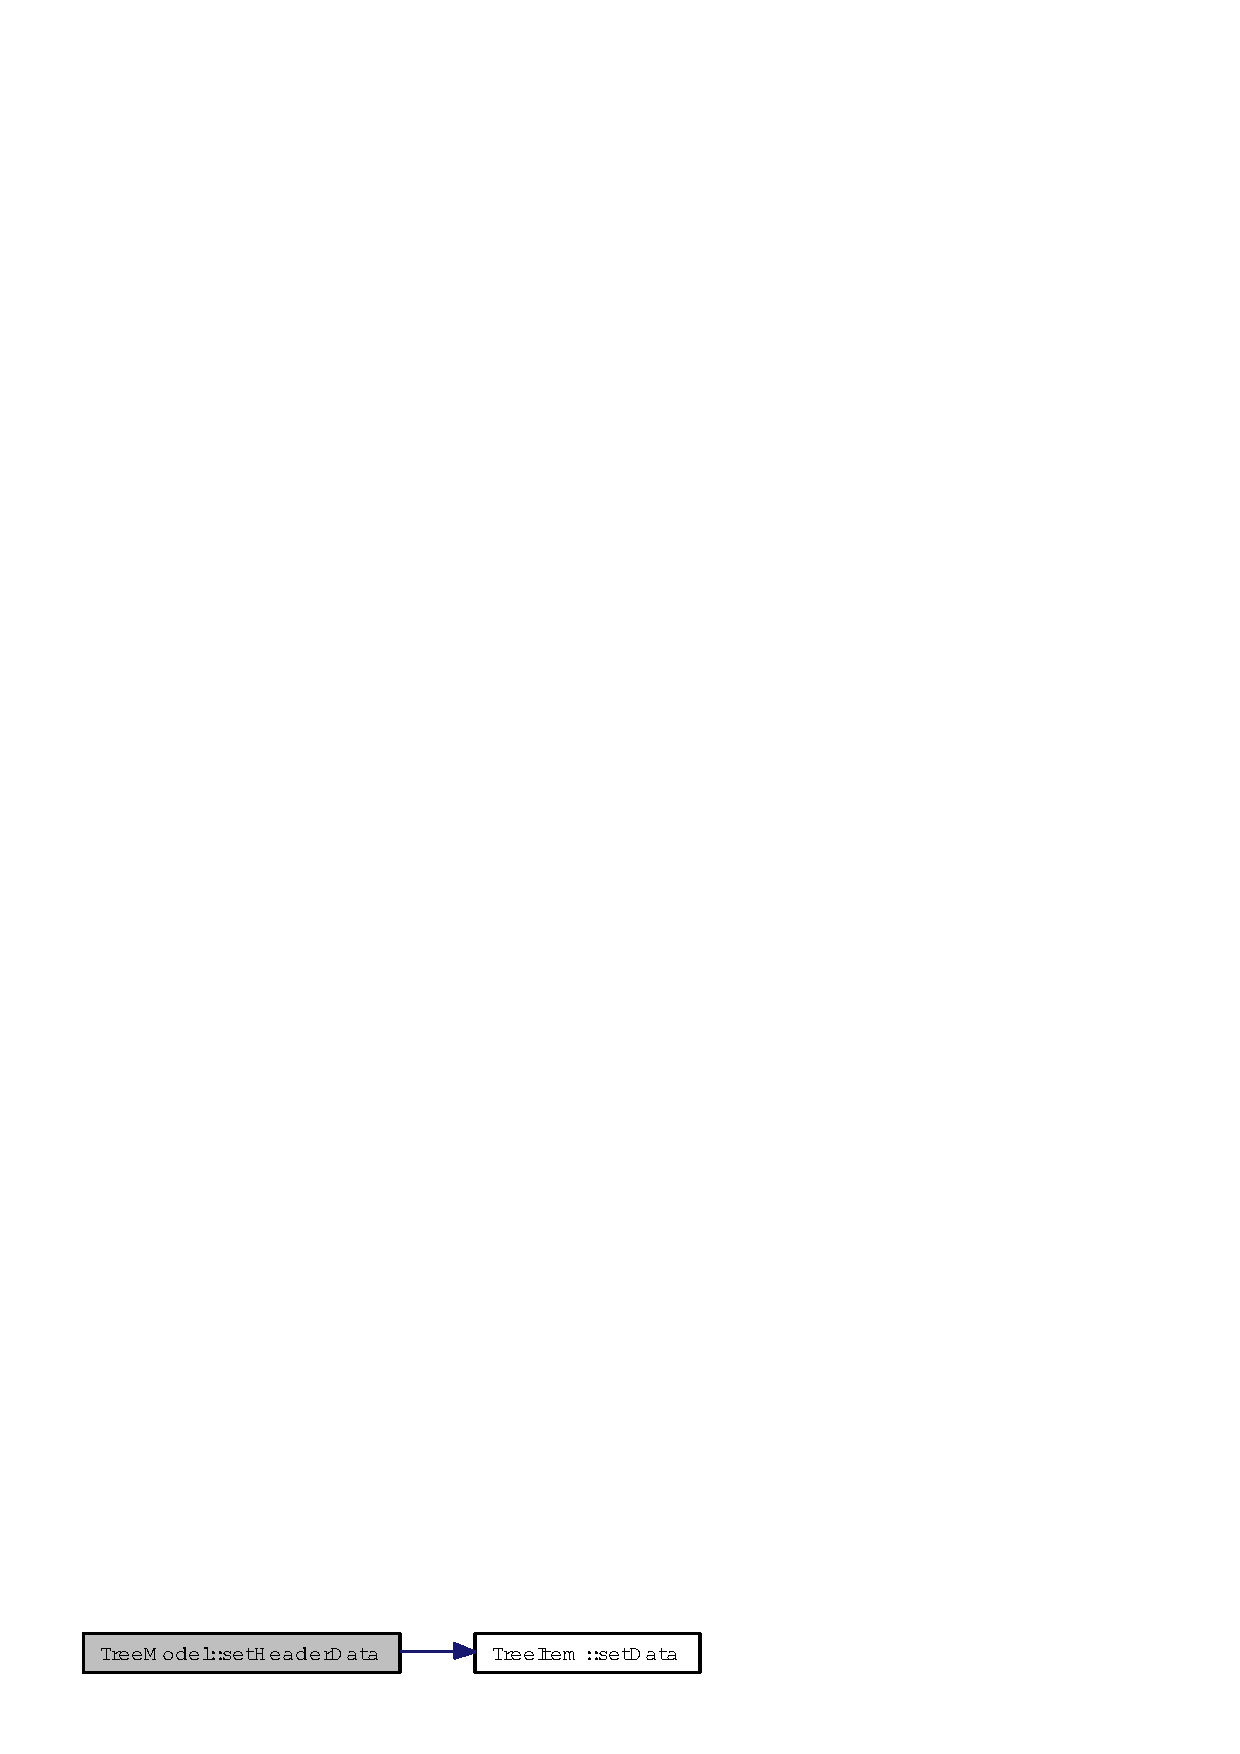
\includegraphics[width=170pt]{classTreeModel_8d42cbbd50936e26241fb6a71ee9fb84_cgraph}
\end{center}
\end{figure}
\index{TreeModel@{Tree\-Model}!insertRows@{insertRows}}
\index{insertRows@{insertRows}!TreeModel@{Tree\-Model}}
\subsubsection{\setlength{\rightskip}{0pt plus 5cm}bool Tree\-Model::insert\-Rows (int {\em position}, int {\em rows}, const QModel\-Index \& {\em parent} = {\tt QModelIndex()})}\label{classTreeModel_56f31919a9eb68ae229afea2257bfc35}




Definition at line 151 of file treemodel.cpp.

References get\-Item(), and Tree\-Item::insert\-Children().

Here is the call graph for this function:\begin{figure}[H]
\begin{center}
\leavevmode
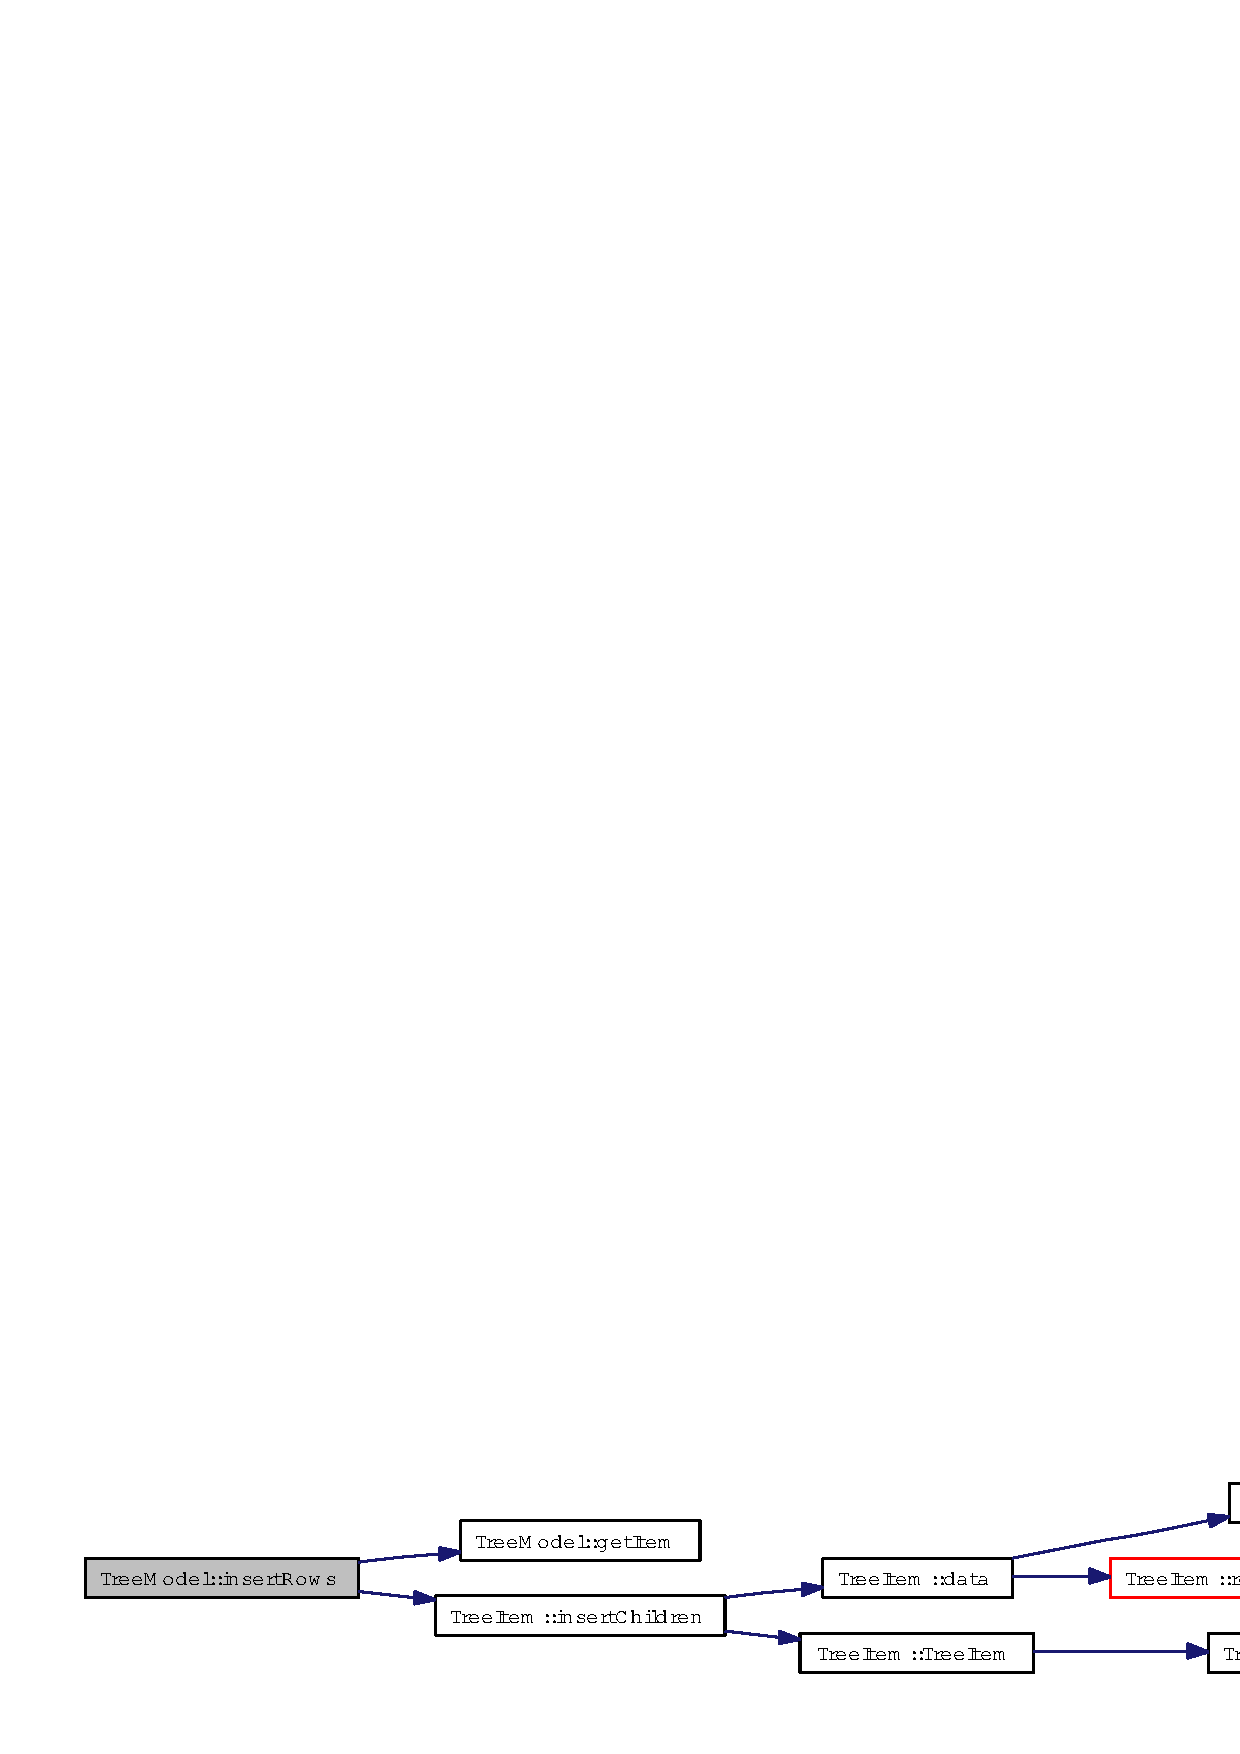
\includegraphics[width=366pt]{classTreeModel_56f31919a9eb68ae229afea2257bfc35_cgraph}
\end{center}
\end{figure}
\index{TreeModel@{Tree\-Model}!removeRows@{removeRows}}
\index{removeRows@{removeRows}!TreeModel@{Tree\-Model}}
\subsubsection{\setlength{\rightskip}{0pt plus 5cm}bool Tree\-Model::remove\-Rows (int {\em position}, int {\em rows}, const QModel\-Index \& {\em parent} = {\tt QModelIndex()})}\label{classTreeModel_592fe71d4120128c096980be4094e87d}




Definition at line 183 of file treemodel.cpp.

References get\-Item(), and Tree\-Item::remove\-Children().

Here is the call graph for this function:\begin{figure}[H]
\begin{center}
\leavevmode
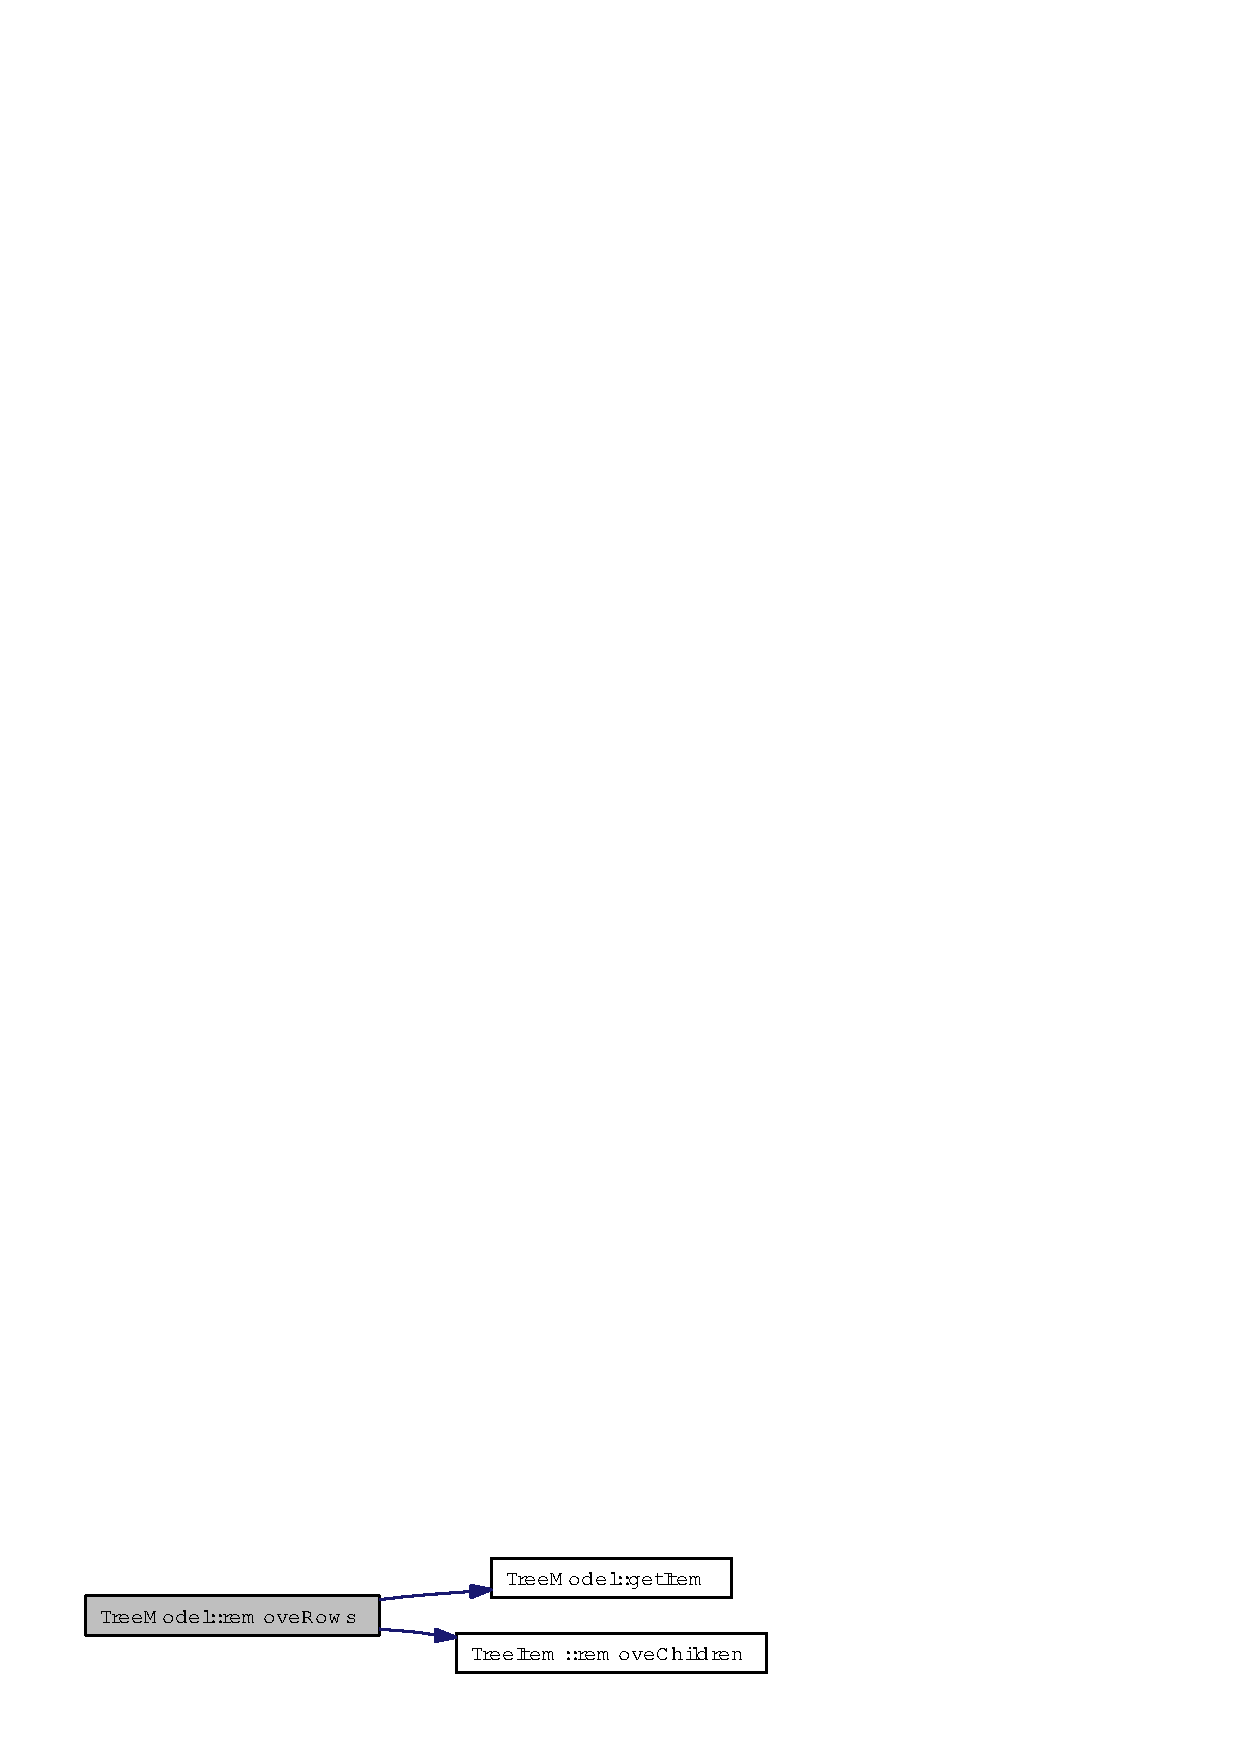
\includegraphics[width=186pt]{classTreeModel_592fe71d4120128c096980be4094e87d_cgraph}
\end{center}
\end{figure}
\index{TreeModel@{Tree\-Model}!getItem@{getItem}}
\index{getItem@{getItem}!TreeModel@{Tree\-Model}}
\subsubsection{\setlength{\rightskip}{0pt plus 5cm}{\bf Tree\-Item} $\ast$ Tree\-Model::get\-Item (const QModel\-Index \& {\em index}) const}\label{classTreeModel_4944fbea068c3d4bc7b25f4a7087b5f0}




Definition at line 68 of file treemodel.cpp.

References root\-Item.

Referenced by knowtreemodel::add\_\-new\_\-child\_\-branch(), knowtreemodel::add\_\-new\_\-sibling\_\-branch(), data(), treescreen::del\_\-branch(), treescreen::edit\_\-branch(), index(), knowtreemodel::index\-Children(), treescreen::ins\_\-branch(), treescreen::ins\_\-subbranch(), insert\-Rows(), knowtreemodel::move\_\-updn\_\-branch(), treescreen::on\_\-knowtree\_\-clicked(), parent(), remove\-Rows(), row\-Count(), mainwindow::save\_\-tree\_\-position(), mainwindow::set\_\-tree\_\-position(), and set\-Data().

Here is the caller graph for this function:\begin{figure}[H]
\begin{center}
\leavevmode
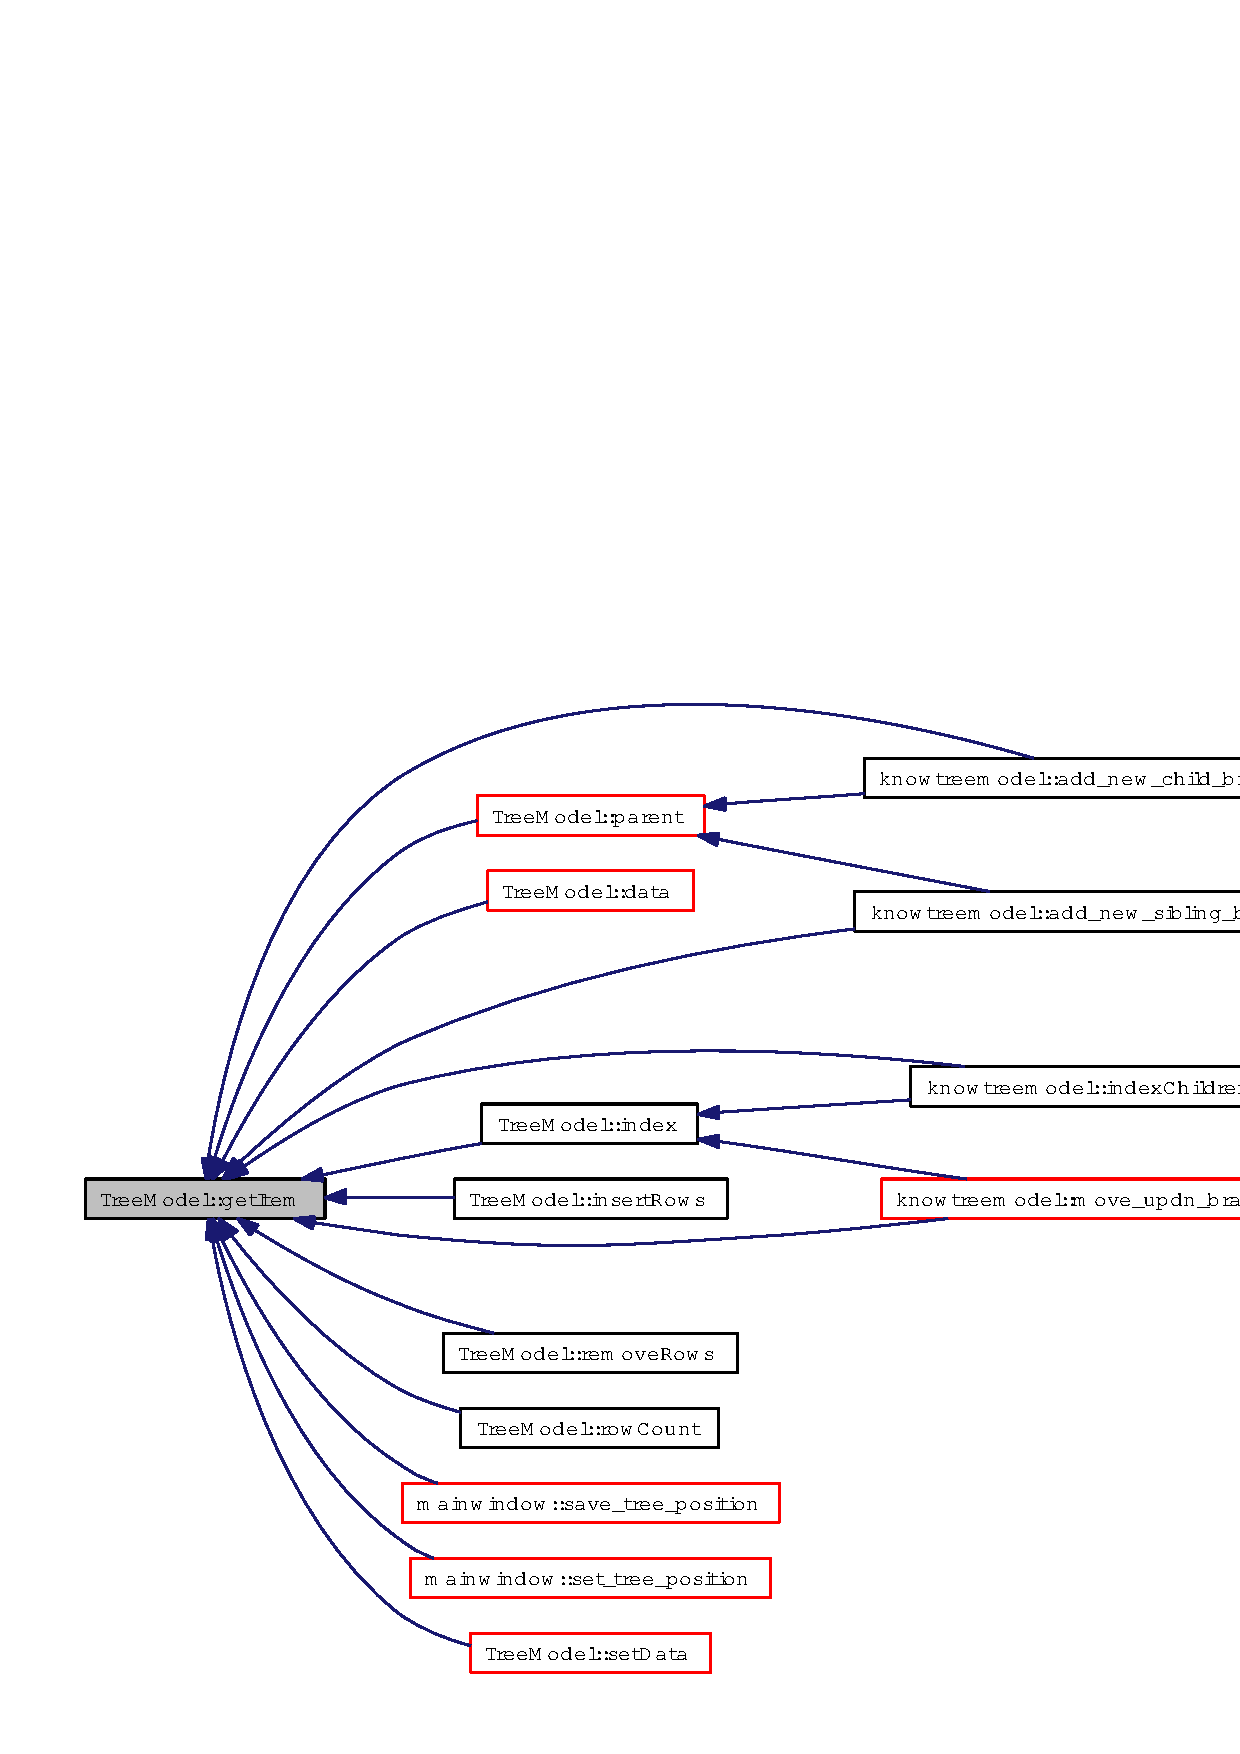
\includegraphics[width=320pt]{classTreeModel_4944fbea068c3d4bc7b25f4a7087b5f0_icgraph}
\end{center}
\end{figure}
\index{TreeModel@{Tree\-Model}!getItem@{getItem}}
\index{getItem@{getItem}!TreeModel@{Tree\-Model}}
\subsubsection{\setlength{\rightskip}{0pt plus 5cm}{\bf Tree\-Item} $\ast$ Tree\-Model::get\-Item (QString\-List {\em path}) const}\label{classTreeModel_eebd988f3ffa0c5b90364be1f9c30eff}




Definition at line 79 of file treemodel.cpp.

References Tree\-Item::child(), Tree\-Item::child\-Count(), critical\_\-error(), data(), and root\-Item.

Here is the call graph for this function:\begin{figure}[H]
\begin{center}
\leavevmode
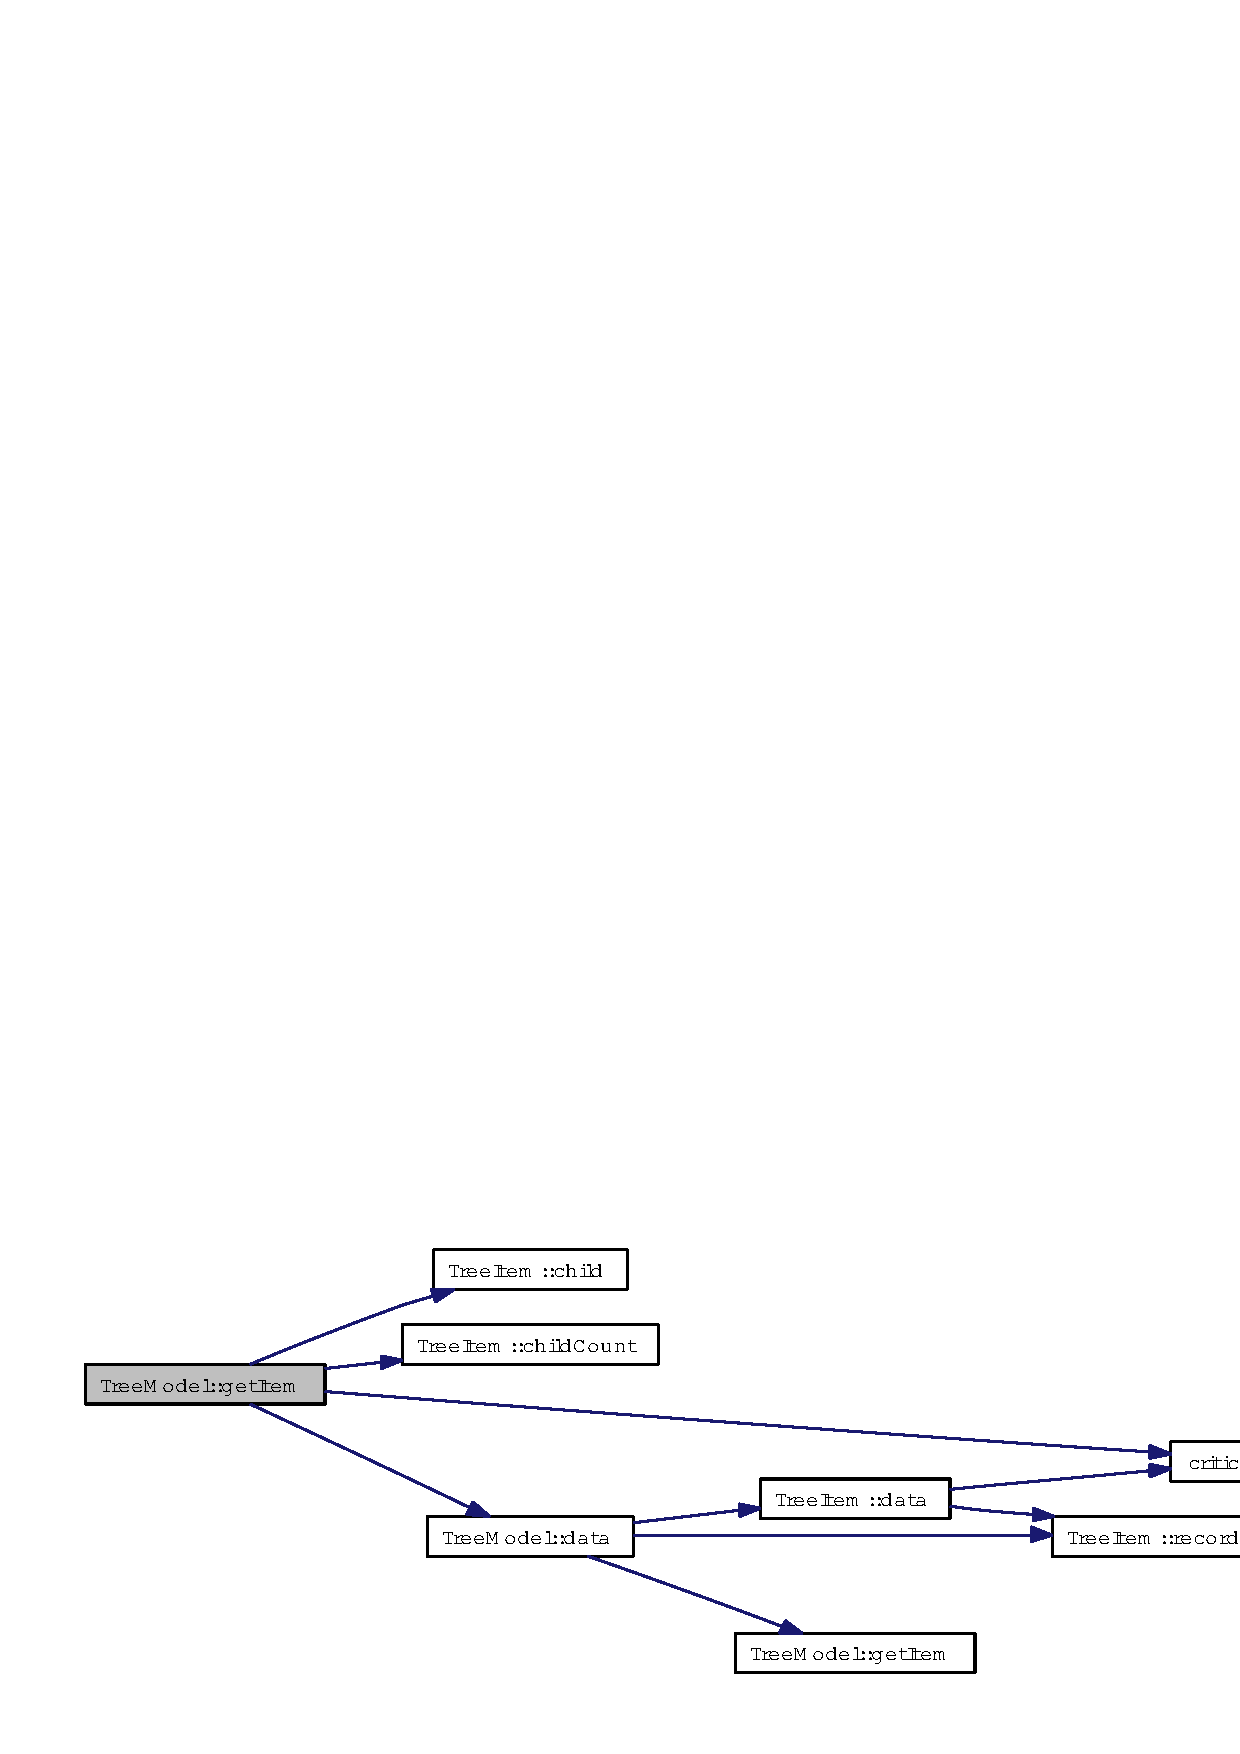
\includegraphics[width=352pt]{classTreeModel_eebd988f3ffa0c5b90364be1f9c30eff_cgraph}
\end{center}
\end{figure}


\subsection{Member Data Documentation}
\index{TreeModel@{Tree\-Model}!rootItem@{rootItem}}
\index{rootItem@{rootItem}!TreeModel@{Tree\-Model}}
\subsubsection{\setlength{\rightskip}{0pt plus 5cm}{\bf Tree\-Item}$\ast$ {\bf Tree\-Model::root\-Item}}\label{classTreeModel_8921084214c2ff8a56b15e201f02ed89}




Definition at line 54 of file treemodel.h.

Referenced by findscreen::find\_\-start(), get\-Item(), knowtreemodel::knowtreemodel(), parent(), treescreen::save\_\-knowtree(), set\-Header\-Data(), and knowtreemodel::$\sim$knowtreemodel().

The documentation for this class was generated from the following files:\begin{CompactItemize}
\item 
{\bf treemodel.h}\item 
{\bf treemodel.cpp}\end{CompactItemize}
